\documentclass[10pt]{article}
\usepackage{graphicx}
\usepackage{hyperref}
\usepackage{amsmath}
\usepackage[shortlabels]{enumitem}
\usepackage{cite}
\usepackage[labelfont=bf]{caption}
\usepackage{float}
\usepackage{listings}
\usepackage{lstautogobble}
\usepackage{adjustbox}
\usepackage{tabularx}
\usepackage[bottom]{footmisc}
\usepackage{indentfirst}

\lstset{basicstyle=\ttfamily,
  mathescape=true,
  escapeinside=||,
  autogobble}

% pretty footnotes
\makeatletter
\renewcommand\@makefntext[1]{\leftskip=2em\hskip-1em\@makefnmark#1}
\makeatother

% wide margins
\addtolength{\oddsidemargin}{-.75in}
\addtolength{\evensidemargin}{-.75in}
\addtolength{\textwidth}{1.5in}
\addtolength{\topmargin}{-.875in}
\addtolength{\textheight}{1.75in}

%%%%%%%%%%%%%%%%%%%%%%%%%%%%%%%%%%%%%%%%%%%%%%%%%%%%%%%%%%%%%%%%%%%%%%%%%%%%%%%%
%~~~~~~~~~~~~~~~~~~~~~~~~~~~~~~~~~~~~~~~~~~~~~~~~~~~~~~~~~~~~~~~~~~~~~~~~~~~~~~%
%%%%%%%%%%%%%%%%%%%%%%%%%%%%%%%%%%%%%%%%%%%%%%%%%%%%%%%%%%%%%%%%%%%%%%%%%%%%%%%%

% STARTING DOCUMENT
\begin{document}

%%%%%%%%%%%%%%%%%%%%%%%%%%%%%%%%%%%%%%%%%%%%%%%%%%%%%%%%%%%%%%%%%%%%%%%%%%%%%%%%
%~~~~~~~~~~~~~~~~~~~~~~~~~~~~~~~~~~~~~~~~~~~~~~~~~~~~~~~~~~~~~~~~~~~~~~~~~~~~~~%
%%%%%%%%%%%%%%%%%%%%%%%%%%%%%%%%%%%%%%%%%%%%%%%%%%%%%%%%%%%%%%%%%%%%%%%%%%%%%%%%

% START TITLE PAGE
\title{\textbf{Kosu: A Decentralized Liquidity Aggregation Primitive}} 
\author{Liam Kovatch, Henry Harder \\\texttt{www.kosu.io}}
\date{\today}
\maketitle
% END TITLE PAGE

%%%%%%%%%%%%%%%%%%%%%%%%%%%%%%%%%%%%%%%%%%%%%%%%%%%%%%%%%%%%%%%%%%%%%%%%%%%%%%%%
%~~~~~~~~~~~~~~~~~~~~~~~~~~~~~~~~~~~~~~~~~~~~~~~~~~~~~~~~~~~~~~~~~~~~~~~~~~~~~~%
%%%%%%%%%%%%%%%%%%%%%%%%%%%%%%%%%%%%%%%%%%%%%%%%%%%%%%%%%%%%%%%%%%%%%%%%%%%%%%%%

%BEGIN ABSTRACT
\begin{abstract}
  \noindent We motivate Kosu, a decentralized network and protocol that encourages the curation of a consistent, high-quality, verifiable, public order book. The Kosu network is a bonded proof-of-stake blockchain built on Tendermint Consensus. The underlying state machine is responsible for enforcing a simple access control ruleset and order booking procedure. The network utilizes a shared security model, wherein all staking and token-based logic is implemented on the Ethereum main network. The model provides unidirectional communication and checkpoints between the two networks by leveraging Tendermint to provide finality for specific Ethereum-based state changes. Individuals intending to post orders to the Kosu network are required to bond tokens for the duration they wish to have access. The poster bonding mechanism creates a market for the allocation of network resources and an implicit incentive to contribute quality liquidity to the network. Kosu validators are selected via a token curated registry system on Ethereum. This registry system allows both the inflation rate as well as the number of active validators to be market driven and determined by the network’s stakeholders. The network is generalizable, supporting orders of arbitrary maker-taker based virtual settlement systems. In its entirety, the proposed system effectively curates a decentralized order book and serves as a liquidity aggregation primitive for second layer systems. Kosu is free to use and open source, reducing barriers to entry for both developers and market agents.
\end{abstract}
\pagebreak
% END ABSTRACT

%%%%%%%%%%%%%%%%%%%%%%%%%%%%%%%%%%%%%%%%%%%%%%%%%%%%%%%%%%%%%%%%%%%%%%%%%%%%%%%%
%~~~~~~~~~~~~~~~~~~~~~~~~~~~~~~~~~~~~~~~~~~~~~~~~~~~~~~~~~~~~~~~~~~~~~~~~~~~~~~%
%%%%%%%%%%%%%%%%%%%%%%%%%%%%%%%%%%%%%%%%%%%%%%%%%%%%%%%%%%%%%%%%%%%%%%%%%%%%%%%%

% TABLE OF CONTENTS
\tableofcontents
\pagebreak
% END TABLE OF CONTENTS

%%%%%%%%%%%%%%%%%%%%%%%%%%%%%%%%%%%%%%%%%%%%%%%%%%%%%%%%%%%%%%%%%%%%%%%%%%%%%%%%
%~~~~~~~~~~~~~~~~~~~~~~~~~~~~~~~~~~~~~~~~~~~~~~~~~~~~~~~~~~~~~~~~~~~~~~~~~~~~~~%
%%%%%%%%%%%%%%%%%%%%%%%%%%%%%%%%%%%%%%%%%%%%%%%%%%%%%%%%%%%%%%%%%%%%%%%%%%%%%%%%

% BEGIN INTRO
\section{Introduction}\label{intro}
Historically, financial markets have been relatively siloed. To date, centralized entities control significant entry points and accounting systems, limiting access beyond a small set of privileged participants\cite{capital-markets-report}. The recent invention of blockchains, decentralized ledger systems, challenges this trusted paradigm. Ethereum, a public blockchain with a built-in Turing-complete programming language, provides developers an immutable and verifiable computation platform for scripts known as ``smart-contracts.'' These scripts can encode arbitrary, deterministic state transition functions, providing a powerful primitive for more complex ledger based application systems\cite{ethereum-whitepaper}.
\medskip

Since the network’s genesis in 2014, developers have leveraged smart contracts for a wide range of novel protocol systems. Perhaps the most adopted technical standard for smart contracts is the ERC-20 token implementation\cite{erc-20}. The standard defines a common token interface allowing for the creation of a diverse set of composable Ethereum-based assets. These tokens often serve as a critical crypto economic primitive providing core utility for protocol systems deployed on Ethereum. As such, a system of exchange is a key requisite for a token-dependent contract ecosystem.
\medskip

In early 2017, the 0x Project published a whitepaper defining a maker-taker based exchange  protocol in which a pipeline of publicly accessible Ethereum smart contracts facilitate the wallet-to-wallet settlement of funds. In this model, order broadcast and discovery happen off-chain. Independent entities known as relayers are responsible for sourcing and maintaining liquidity in the form of signed order messages. This hybrid architecture drastically improved the efficiency of existing decentralized exchange (DEX) systems while also providing a critical open exchange primitive with high extensibility\cite{0x-wp}. Since the first deployment of the 0x protocol, a significant number of projects have adopted it as a common piece of infrastructure facilitating 713,000 trades and \$750,000,000 in volume at the time of writing. Moving forward, the team continues to innovate on the scalability, efficiency and incentivization of DEX systems.
\medskip

Virtual settlement systems, specifically decentralized exchanges, are a relatively accessible use case for blockchains; a direct evolution from the original digital currency use-case. While conceptually apparent, the architecture of DEXs is a complex and evolving subject. The scalability constraints of blockchain systems combined with the complexities of an asynchronous discrete time system limit their compatibility with continuous time order books and settlement systems\cite{flash-boys-2}. As such, alternative DEX architectures have also captured considerable market share. These systems include dutch auctions and automated market making systems. While immediately compelling for some use cases, the evolution towards hybrid decentralized exchange structures, similar to 0x, is likely. These systems, though currently constrained, have a clear path towards scalability and offer the most competitively priced and extensible DEX structure to date\cite{0x-roadmap-pt-2}. 
\medskip

The Kosu network is designed within the 0x-motivated ecosystem, providing a decentralized aggregation primitive for arbitrary limit orders. More specifically, the Kosu network aims to provide a highly extensible decentralized complement to independent centralized aggregators, or relayers. The set of orders maintained on the Kosu network will represent a high-value subset of the available order universe.
\clearpage
\pagebreak
% END INTRO

%%%%%%%%%%%%%%%%%%%%%%%%%%%%%%%%%%%%%%%%%%%%%%%%%%%%%%%%%%%%%%%%%%%%%%%%%%%%%%%%
%~~~~~~~~~~~~~~~~~~~~~~~~~~~~~~~~~~~~~~~~~~~~~~~~~~~~~~~~~~~~~~~~~~~~~~~~~~~~~~%
%%%%%%%%%%%%%%%%%%%%%%%%%%%%%%%%%%%%%%%%%%%%%%%%%%%%%%%%%%%%%%%%%%%%%%%%%%%%%%%%

% BEGIN OVERVIEW SECTION
\section{Overview}\label{overview}
Kosu is a public blockchain designed to support the construction of order booking and liquidity systems for emerging decentralized financial primitives. The Kosu network uses a bonded proof-of-stake security model implemented with Tendermint Consensus\cite{tendermint} and a system of Ethereum contracts that include the protocol’s native token.
\medskip

Kosu is primarily composed of two interdependent systems\footnote{\ These systems are described in more detail in section \ref{specification}.} that together implement the protocol’s core function: to establish and curate a consistent and verifiable set of recent, high-quality orders. The Kosu contract system is responsible for defining the protocol's incentive mechanisms, facilitating validator curation by stakeholders, and specifying an access control scheme for the Kosu network. The functionality provided by the contract system supports the network-based order booking service upon which exchange and liquidity systems can be built.
\medskip

The Kosu network is a system of globally distributed nodes that collectively maintain and update the shared order book\footnote{\ The Kosu order book is a set of hashes of specific recent orders, from which conventional limit order books can be constructed. See section \ref{tm-network-state}.} and blockchain while providing a one-way peg to Ethereum. The network supports basic order booking functionality, access control for user accounts, and cryptographic proofs of the existence of state contents, including the set of orders that compose the current ``order book.'' Validators\footnote{\ Kosu non-validating full nodes crucially provide access to the order book and enable users to submit orders, laying the foundation for a wide array of applications. Full nodes also allow a wide variety of proofs to be constructed about the existence or absence of state data.} secure the network by submitting attestations about specific state changes to the Ethereum contract system, processing orders, and reaching consensus on the canonical chain and overall application state. 
\medskip

The Kosu protocol’s Ethereum-based smart-contract system implements the protocol’s native token and core incentive mechanisms. These mechanisms manage access control for posters and allow stakeholders to curate the Kosu network’s validator set through a novel weighted voting system and token-curated registry.
\medskip

Kosu validators are required to run full Ethereum nodes and are responsible for submitting special attestations, or ``witness'' transactions, to the Kosu network about specific state changes to the protocol’s contract system. Specifically, the network must reflect updates to users’ bonded token balances (which affect a order rate limit enforced by the network), and updates to the dynamic registry contract containing the curated list of validators.
\medskip

Individuals who wish to leverage the network’s decentralized order booking and message relay features are called posters, and can gain write access to the network by bonding any amount of Kosu tokens in a poster registry contract. After their bond transaction is confirmed on Ethereum to a certain depth, validators update the Kosu network's shared state to reflect the bonded balance change of the new poster. The same mechanism allows posters to adjust the amount of tokens they have bonded, or withdraw entirely from the system at any time. The amount of tokens a poster chooses to bond determines the maximum number of orders they may post per defined period, which is proportional to their bonded balance relative to the total number tokens bonded by posters.
\medskip

At deterministic intervals based on the height of the Ethereum blockchain, Kosu validators compute a simple rate-limit mapping based on in-state balance data that allocates network order throughput proportionally to posters who have Kosu tokens bonded at the height a new interval starts. These intervals are called rebalance periods and allow the relatively continuous process of balance updates on the Ethereum Poster Registry, as a result of bonding/unbonding by posters, to be mapped to more discrete periods of rate-limiting in a deterministic manner. At the beginning of each new rebalance period, validators must reach consensus on the parameterization of the upcoming period. The starting and ending Ethereum block heights of the period, and the total number of orders to be accepted from posters during that time is determined prior to allowing posters write access for the period.
\medskip

During normal network operations between rebalance periods, validators accept and process incoming order transactions from posters (gossiped via connected full nodes), while submitting regular attestations (called witness transactions) to other validators on the network. This process ensures the state of the Kosu Ethereum contract system is accurately tracked.
\medskip

The validity of order transactions is based on the signature of the poster that submitted the order to the network, and a certain required data structure that enables recovery of the signature. An order is considered valid if it contains a recoverable signature from a poster account with a non-zero remaining order post limit for the current rebalance period. Validators will include such orders in a block and decrement the posters bandwidth allocation limit for that period for each order submitted. 
\medskip

The Kosu network uses a bonded proof-of-stake security model wherein validators stake (by locking) tokens into a contract proportional to the amount of vote power they wish to receive on the network. The number of tokens they associate with their stake are locked for the duration the entity wishes to validate. The validator may be stripped of their power at any time at the discretion of voting token holders, and if voted out, their tokens are distributed to the individuals responsible for raising – and voting in – the successful challenge. 
\medskip

During the continuous validator governance and curation process, individuals wishing to become validators submit proposals in which they specify a positive or negative reward schedule. If this value is positive, the validator will be rewarded newly minted tokens that inflate the existing supply. If the value is negative, validators will be required to constantly collateralize their listing at the rate specified so their tokens may be burned. In this case, the negative ``reward'' deflates the existing supply. 
\medskip

The ability for validators to specify both negative and positive reward rates is a crucial component of the overall system design. For the nascent network, validators will be able to extract little value from the act of validating alone, thus will require inflationary rewards that justify the costs of managing validator infrastructure. However, in a mature state the Kosu network could present implicit value capture opportunities to validators in the form of positional information advantages. More generally, validator reward schedules are market-driven and account for both implicit and explicit reward capture.

\clearpage
\pagebreak
\subsection{Usage example}\label{overview-example}
\begin{figure}[H]
  \centering
  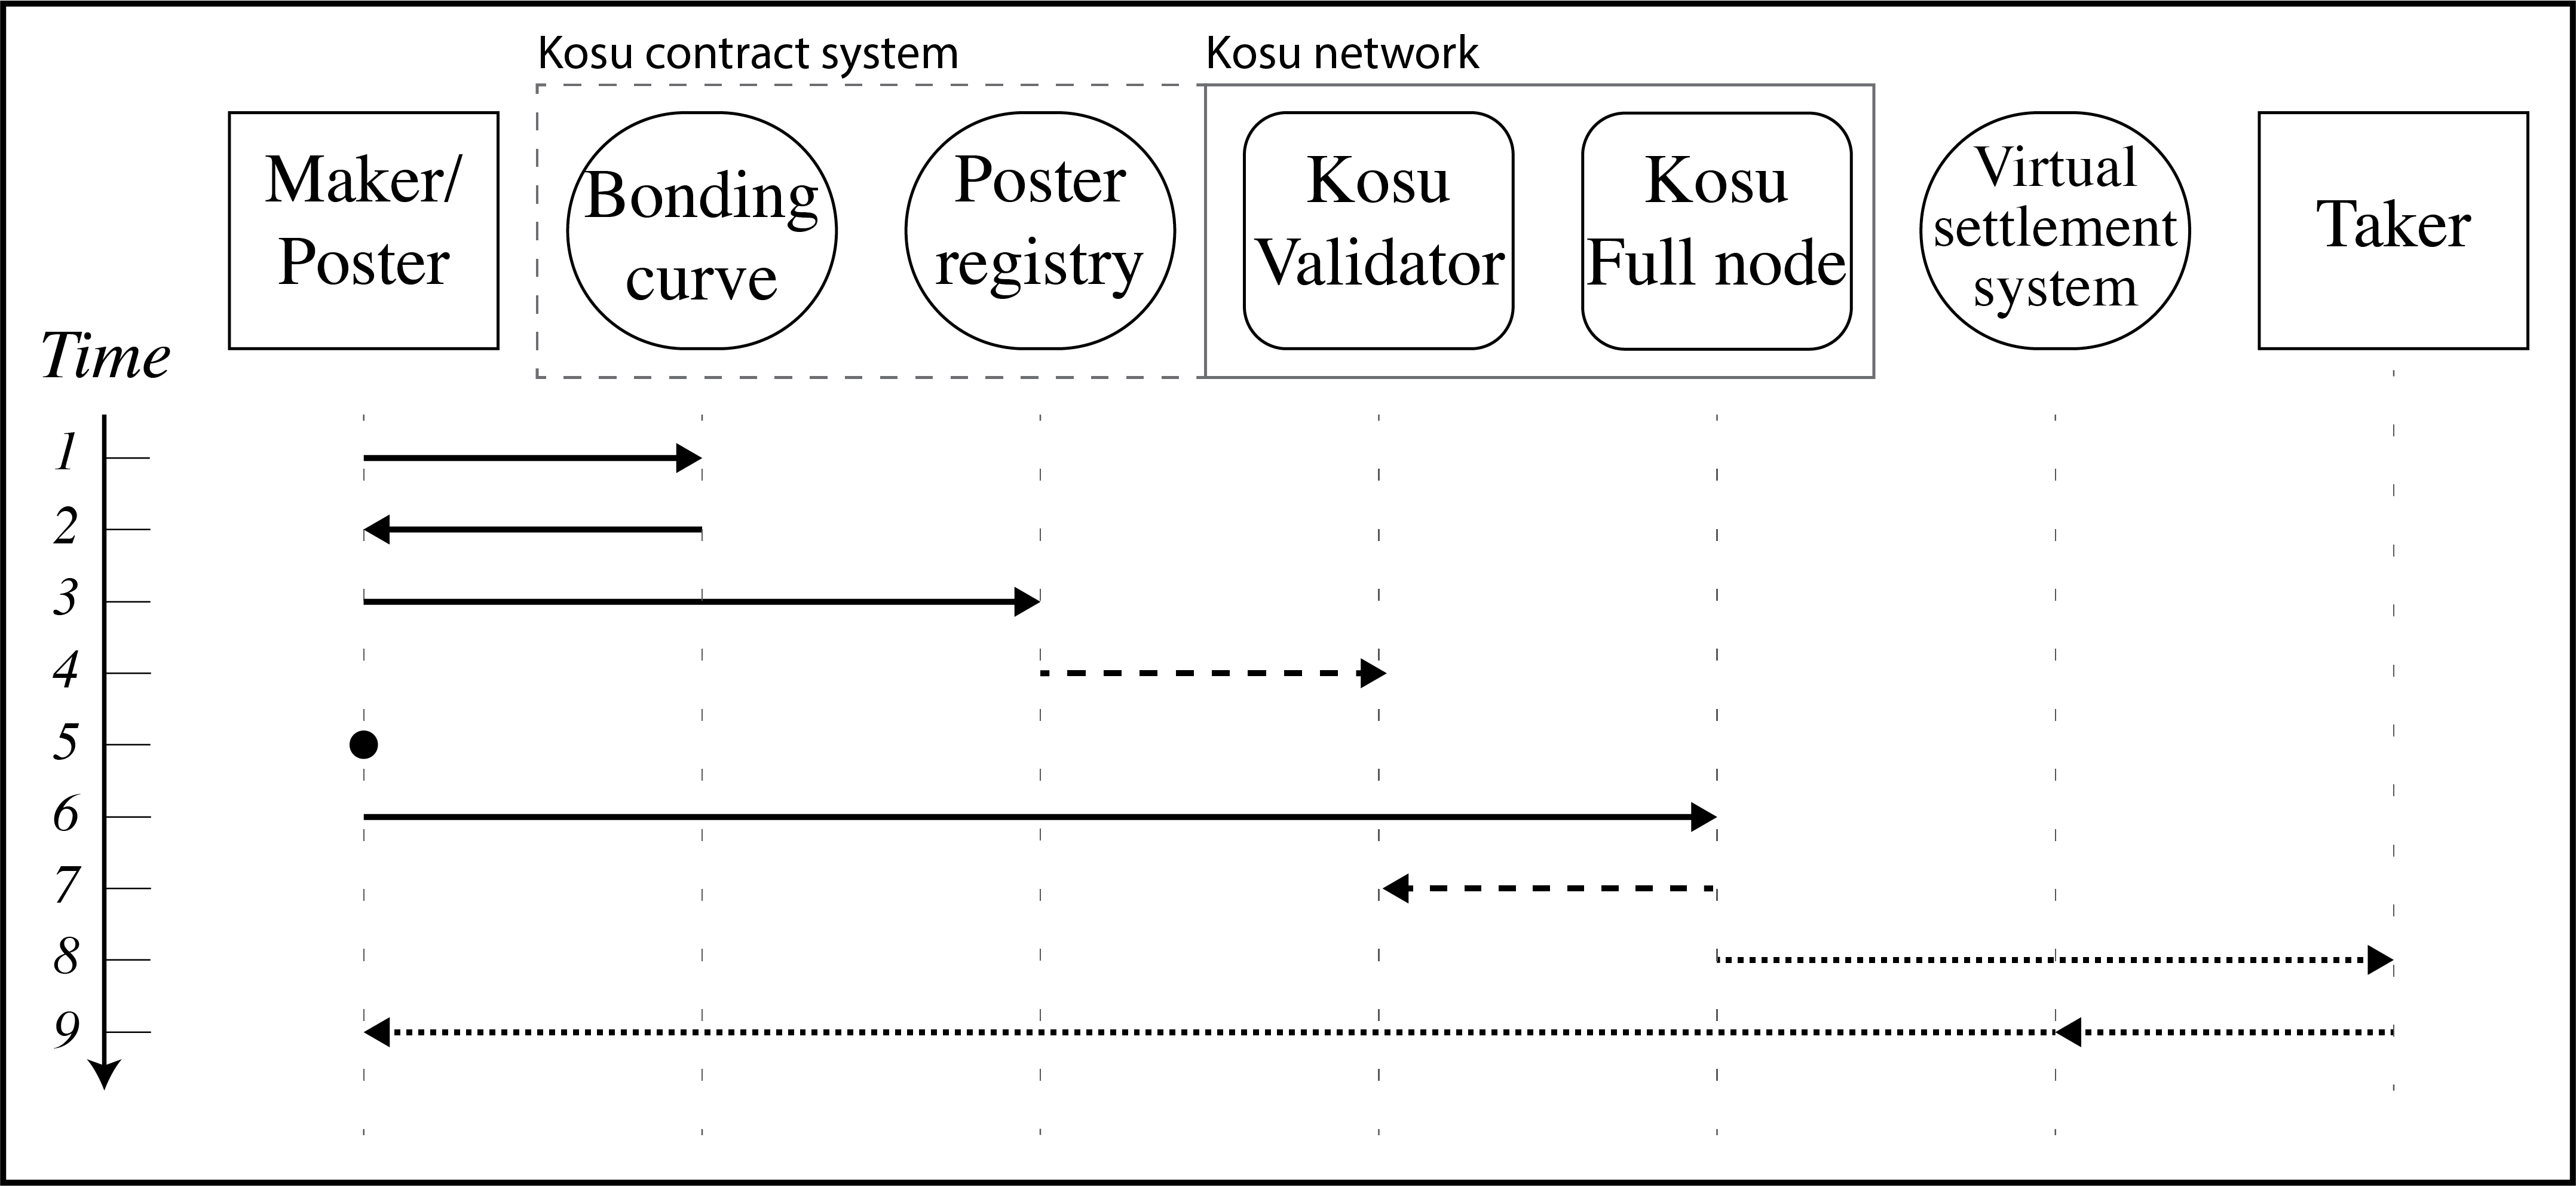
\includegraphics[width=\textwidth]{../figures/fig2.png}
  \caption{Simplified chronology (arranged with time progressing in the downward direction) of the steps involved for a new user (the poster) to submit an order to the Kosu network. The individual time-steps are shown on the left (and annotated below), with the first action taking place at time-step 1.}
  \label{fig:fig1}
\end{figure}
Figure \ref{fig:fig1} illustrates the actors, systems, and procedures involved in enabling a new user (the ``poster'') to contribute liquidity, via a signed order message, to the Kosu network and order book. 
\medskip

Boxes represent individuals or human-controlled actors, ovals represent Ethereum smart-contracts, and boxes with rounded corners represent Kosu nodes. Solid arrows and dots indicate actions triggered by the poster, dashed arrows represent interactions validators are responsible for, and dotted arrows represent actions triggered by the ``taker,'' the individual or entity who fills the poster's order by submitting it to a virtual settlement system (such as the 0x protocol\cite{0x-wp}).
\medskip

\begin{enumerate}[1.]
  \item A poster who intents to contribute liquidity to the Kosu network ``buys'' KOSU tokens by locking an arbitrary amount of Ether in the token's bonding curve contract.
  \item In the bond transaction, the contract ``sends'' KOSU tokens to the poster according to the bonding curve equation and its current parameterization.
  \item The poster bonds any amount of their new KOSU tokens in the Poster Registry contract
  \item The Kosu/Ethereum peg-zone updates the poster's balance in the Kosu network's shared state, granting them write access to the order book.
  \item The poster creates and signs a maker order message for an arbitrary settlement system, indicating their intent and ability to trade.
  \item The poster submits their order message as a transaction to the Kosu network via a full node (or light client).
  \item A Kosu validator includes the order transaction in a block and makes the order available to the greater network.
  \item A taker (any individual filling maker order messages by submitting them for settlement) becomes aware of the new order from their own Kosu full node or light client.
  \item The taker submits the maker order and any additional required information to an arbitrary blockchain-based virtual settlement system (such as 0x) according to the maker order's type. In most cases, the settlement system will initiate some type of transfer of funds between the maker and the taker.
\end{enumerate}
\clearpage
\pagebreak
% END OVERVIEW SECTION

%%%%%%%%%%%%%%%%%%%%%%%%%%%%%%%%%%%%%%%%%%%%%%%%%%%%%%%%%%%%%%%%%%%%%%%%%%%%%%%%
%~~~~~~~~~~~~~~~~~~~~~~~~~~~~~~~~~~~~~~~~~~~~~~~~~~~~~~~~~~~~~~~~~~~~~~~~~~~~~~%
%%%%%%%%%%%%%%%%%%%%%%%%%%%%%%%%%%%%%%%%%%%%%%%%%%%%%%%%%%%%%%%%%%%%%%%%%%%%%%%%

% BEGIN TECH SPEC SECTION
\section{Specification}\label{specification}
The specification for each system in this section serves to communicate the purpose and functionality of each component, rather than provide a fully accurate description of specific implementation details.
\medskip

Many nuanced components and processes are referenced at a high level for the sake of brevity and digestibility. Each component of the protocol’s implementation is open source and should be referred to for the most detailed and up-to-date specification and implementation\cite{paradigm-github}.
%%%%%%%%%%%%%%%%%%%%%%%%%%%%%%%%%%%%%%%%%%%%%%%%%%%%%%%%%%%%%%%%%%%%%%%%%%%%%%%%
% BEGIN ORDER SPECIFICATION SUB-SECTION
\subsection{Orders}\label{orders}

The Kosu protocol defines a simple and extensible data structure to represent signed order messages on the network. The primary purpose of the defined order schematic is to allow signature recovery for the verification of poster bandwidth allocation during order processing and validation.
\medskip

The order format described below is also designed to allow the ``wrapping'' of existing hybrid-decentralized\footnote{\ Refers to DEX architecture where asset settlement takes place on-chain, and order matching/relay occurs elsewhere.} order messages (such as 0x and Dharma\cite{0x-wp, dharma-wp}) for relay on the Kosu network, and settlement through a system of generalizable forwarding contracts.
\medskip

Usage of the forwarding contract system is strictly optional, and unrelated to the core protocol in the sense that no state is shared between the protocol contract system and settlement contracts (called SubContracts, defined below).

\subsubsection{SubContract interface}\label{subcontract-interface}

Kosu can act as an order message aggregator and/or transport layer for a variety of types of on-chain exchange systems. To achieve this, a simple and extensible contract-based interface is defined that allows a common order message format to be used for a variety of Ethereum settlement pipelines that leverage hybrid decentralized exchange architecture.
\medskip

All current SubContract implementations are in Solidity and designed for use with Ethereum, however, any language and blockchain that supports sufficient scripting capabilities to satisfy the interface described in the table below can be used with Kosu\footnote{\ Posters must provide RLP-encoded SECP256K1 signatures in orders submissions regardless of settlement type.}.
\medskip

% Begin table 1
\bgroup
\def\arraystretch{1.2}
\begin{table}[H]
\centering
\label{table:table1}
\begin{tabularx}{1\textwidth}{|l|l|X|p{8cm}|}
\hline
\textbf{Method name} & \textbf{Returns} & \textbf{Params.} & \textbf{Description} \\ 
\hline
\texttt{makerArguments} & \texttt{string} & \texttt{-} & Returns a JSON string containing a data structure that specifies the required fields for maker orders for the SubContract. \\
\hline
\texttt{takerArguments} & \texttt{string} & \texttt{-} & Returns a JSON string containing a data structure (identical to \texttt{makerArguments}) that specifies the values a taker must supply when filling a maker order. \\
\hline
\texttt{isValid} & \texttt{boolean} & \texttt{makerData} & Checks weather a maker order is valid and fillable based on the SubContract's validation implementation \\
\hline
\texttt{amountRemaining} & \texttt{uint256} & \texttt{makerData} & For settlement types that support it, this method can return information that allows partial fills \\
\hline
\texttt{participate} & \texttt{boolean} & \texttt{makerData}, \texttt{takerData} & The main settlement logic implementation for SubContracts, which triggers execution of a trade by the taker submitting the maker data and their counter-party information. \\
\hline
\end{tabularx}
\caption{Describes the SubContract interface and method signatures in a language-independent manner.} 
\end{table}
\egroup
% End table 1

Some of the data structures used by the \texttt{SubContract} interface and Kosu order message structure are described in more detail below. The full interface definition in Solidity can be found on the \texttt{ParadigmFoundation} GitHub\cite{kosu-sdk}.

\begin{itemize}
  \item \texttt{makerArguments}: a structure that defines the name and types of each argument in the \texttt{makerValues}
  \item \texttt{takerArguments}: defines the arguments (name and type) takers must provide to \texttt{participate} 
  \item \texttt{makerData}: an array of 32 byte slices of serialized data included in the maker order message
  \item \texttt{takerData}: an array of 32 byte slices of serialized data provided by the taker as arguments
\end{itemize}

Since validity conditions of a given order vary greatly between settlement systems, a generic validation interface method (\texttt{isValid}) is provided. A method that returns an arbitrary integer (\texttt{amountRemaining}) is also specified, which can be used to support partial fills for settlement types where it is logical, such as spot exchange implementations.

\subsubsection{Order message format}\label{order-message-format}

A simple order message format is defined based on the SubContract interface. The data structure was specifically designed to satisfy the following requirements:

\begin{enumerate}
  \item Compatibility with new and existing hybrid off-chain settlement systems (0x, Dharma, etc.\cite{0x-wp, dharma-wp})
  \item Efficient and lossless compression with existing transports and multiple languages in mind.
  \item Support for serialization to EVM compatible data types and structures.
  \item Support for arbitrary signature schemes\footnote{\ All orders still must include an SECP256K1 signature from a poster Ethereum account with bonded Kosu tokens.} within maker order messages
\end{enumerate}

The Kosu order message format is described below in a language-agnostic manner, however the type annotations indicate the JSON type each top-level field is serialized to. The underlying structure of the non-primitive types (\texttt{array} and \texttt{object}) are defined in the protocol's implementation\cite{kosu-monorepo} and documentation.

% Begin table 2
\bgroup
\def\arraystretch{1.2}
\begin{table}[H]
\centering
\label{table:table2}
\begin{tabularx}{1\textwidth}{|l|l|l|X|}
\hline
\textbf{Field name} & \textbf{Type} & \textbf{Required} & \textbf{Description} \\
\hline
\texttt{subContract} & \texttt{string} & yes & The deployed address of the target SubContract settlement implementation. Defines expected arguments. \\
\hline
\texttt{maker} & \texttt{string} & yes & The address of the party that signed the maker order. Usually indicates the beneficiary of settled funds. \\
\hline
\texttt{makerArguments} & \texttt{array} & no & An array of equal length to the number of \texttt{makerArguments} containing objects that define the name and data-type for each argument. \\
\hline
\texttt{takerArguments} & \texttt{array} & no & Similar to \texttt{makerArguments}, it defines the values and data-types required for settlement. Not required for maker orders. \\
\hline
\texttt{makerValues} & \texttt{object} & yes & A hash-map data structure that contains the parameters necessary for a valid maker order of the target settlement type. \\
\hline
\texttt{makerSignature} & \texttt{object} & no & An optional field that can be used to include a signature from the maker. May also be included in \texttt{makerValues}. \\
\hline
\texttt{posterSignature} & \texttt{object} & yes & Stores the signature resulting from a poster entity signing a hash of the maker order values. Used to verify poster has bonded tokens. \\
\hline
\end{tabularx}
\caption{Generic and high-level description of the Kosu order message format, including optional fields.} 
\end{table}
\egroup
% End table 2
% END ORDERS SUB-SECTION
%%%%%%%%%%%%%%%%%%%%%%%%%%%%%%%%%%%%%%%%%%%%%%%%%%%%%%%%%%%%%%%%%%%%%%%%%%%%%%%%

%%%%%%%%%%%%%%%%%%%%%%%%%%%%%%%%%%%%%%%%%%%%%%%%%%%%%%%%%%%%%%%%%%%%%%%%%%%%%%%%
% BEGIN ETHEREUM CONTRACT SYSTEM SUB-SECTION
\subsection{Ethereum Contract System}\label{ethereum-contract-system}
\subsubsection{Introduction}\label{ethereum-contract-system-intro}
The Kosu protocol implementation includes a suite of Ethereum contracts that are responsible for a set of core functionalities related to access control (sybil tolerance), network validator governance, and the protocol’s core economic mechanisms (described in detail in section \ref{incentive-models}).
\medskip

The contract system allows the primary users and stakeholders of the system to participate in governance of the active validator set, manage their Kosu token balances and allowances, and/or gain write access to the Kosu order book.
\medskip

Specific components of the overall contract system leverage proxy contracts to provide external interfaces to system components, while allowing the actual implementation contract to be replaced if network stakeholders ever deem such action necessary.
\medskip

The Kosu token\footnote{\ The KOSU token implements the ERC-20 standard interface\cite{erc-20}}, the protocol's native asset, is a component of the Ethereum contract system. The token is used throughout the protocol (via the contract system) to allocate resources on the Kosu network (see \ref{tm-network} and \ref{incentive-models}), as the asset validators must stake, and to incentivize the curation of a high-quality validator set (see \ref{ethereum-contract-system-tcr} and \ref{incentive-models-validators}).  
\medskip

The contract system is modular and designed with upgradability in mind. Due to the permanence of smart contracts, the ability to deploy upgrades and additions to existing contract systems is limited, unless specific consideration is made during the system’s design. Kosu’s architecture allows such upgrades and additions to the system (with stakeholder approval\footnote{\ See the future work section for details on the transition to general stakeholder governance.}) through the use of proxy contracts and a mutable authorization registry contract for managing the system’s internal permissions.

\subsubsection{Architecture}\label{ethereum-contract-system-architecture}
The Kosu contract system uses a system of public-facing\footnote{\ The proxies are intended to be the interface points with the system, while no meaningful interactions are possible with implementation contracts.} proxy contracts that perform calls to independent implementation contracts where the primary logic and state management resides.
\medskip

Authorization of internal system methods (including management of the validator set and token supply), is managed by a registry contract that contains the addresses of protocol contracts that are permissioned to access those methods.
\medskip

Such an architecture is desirable primarily for the following reasons:

\begin{enumerate}
  \item A component implementation may be updated while the proxy contract's address stays the same\footnote{\ In order for this to be true, there must be no breaking changes to the component's interface.}.
  \item Implementation contracts can operate in ``trusted environments'' by only accepting calls from the designated proxy.
\end{enumerate}

\subsubsection{System components}\label{ethereum-contract-system-components}
Below is a list of the primary components (contracts) that make up the overall Kosu contract system, and a brief description of the functionality of each. More detail is provided about certain components in the following subsections.

\begin{itemize}
  \item \texttt{AuthorizedAddresses} - a registry containing the addresses of certain protocol contracts. Enables a method modifier (\texttt{isAuthorized}) to restrict access to internal and sensitive methods.
  \item \texttt{Authorizable} - implements a method modifier that restricts callers to addresses in the authorization registry (\texttt{AuthorizedAddresses}), inherited by many protocol contracts.
  \item \texttt{EventEmitter} - a contract responsible for emitting all system event logs. It is used by the Witness component of the Ethereum peg zone (see \ref{peg}).
  \item \texttt{KosuToken} - an implementation of the ERC-20 interface and the protocol's native token.
  \item \texttt{Treasury} - central contract that manages system accounting and allowances, and other functionality related to balances and token supply.
  \item \texttt{PosterRegistryProxy} - the proxy contract for the \texttt{PosterRegistry} that provides its external (public) interface.
  \item \texttt{ValidatorRegistryProxy} - the proxy contract for the \texttt{ValidatorRegistry} that provides the public interface for validator governance and voting mechanisms.
  \item \texttt{PosterRegistry} - implementation contract that allows users to bond\footnote{\ The term ``stake'' is avoided here since the balance may not be slashed, and does not provide explicit rewards for lockup.} and un-bond KOSU tokens at arbitrary times and amounts in exchange for write access to the Kosu network order book. 
  \item \texttt{ValidatorRegistry} - an implementation of a modified token-curated-registry\cite{tcr-1} that allows any KOSU token holder to participate in the selection of the Kosu network's validators. Stakeholders are rewarded for participating in governance (for certain outcomes) by challenging new and existing listings, and voting on those challenges. 
  \item \texttt{Voting} - implementation contract that manages challenges and votes for the \texttt{ValidatorRegistry} contract. Implements a basic commit-reveal voting scheme.
\end{itemize}

The only contracts that provide meaningful functionality for external users are the Treasury, KOSU token contract, and the registry proxies for posters, validators, and voters.

\subsubsection{Treasury}\label{ethereum-contract-system-treasury}
The Treasury contract is responsible for managing system token allowances, executing adjustments to token supply (as a result of the validator reward process), and other functionality related to asset management within the Kosu contract system.
\medskip

It acts as a central accounting system and tracks the balances of users' tokens throughout the system, including those bonded by posters, staked by validators, or idly deposited within the treasury. This accounting system is crucial to the systems voting mechanics, which relies of the Treasury’s account of each user’s total system balance to assign vote power to participating stakeholders. 
\subsubsection{Poster bonding}\label{ethereum-contract-system-poster-bonding}
The Poster Registry contract is a simple registry system that allows users to bond (register) and un-bond (release) Kosu tokens at any time, and in arbitrary amounts. The contract maintains a mapping of accounts to bonded token balances, and importantly, triggers the emission of an event log through the EventEmitter contract each time a poster registers or releases tokens, including the account address and the new balance.
\medskip

Generation of the rate-limit mapping that allocates network order throughput (see \ref{tm-network-access}) to posters is handled by the Kosu network, after balance updates to the contract system are reflected in the network's shared state. This process, described in section \ref{peg}, is part of Kosu’s Ethereum peg-zone.
\subsubsection{Validator token-curated registry}\label{ethereum-contract-system-tcr}
The Validator Registry contract is an implementation of a token-curated registry (TCR), and a cornerstone piece of the Kosu protocol that enables decentralized curation of the networks validator set.

The goal of a TCR is to produce a curated set of \textit{listings}, which are entries that have successfully been included in the registry. Listings begin as \textit{proposals} which indicate intent to join the registry, backed by a number of tokens. Proposals and listings may be \textit{challenged} at any time, where a challenger must put up an equal number of tokens as the listing or proposal owner. Challenges trigger votes, which any token holder may participate in. 
\medskip

The specific mechanics of listings, proposals, and challenges within the Kosu Validator Registry are illustrated in figure \ref{fig:fig3} described below. 
\medskip

\begin{figure}[H]
  \centering
  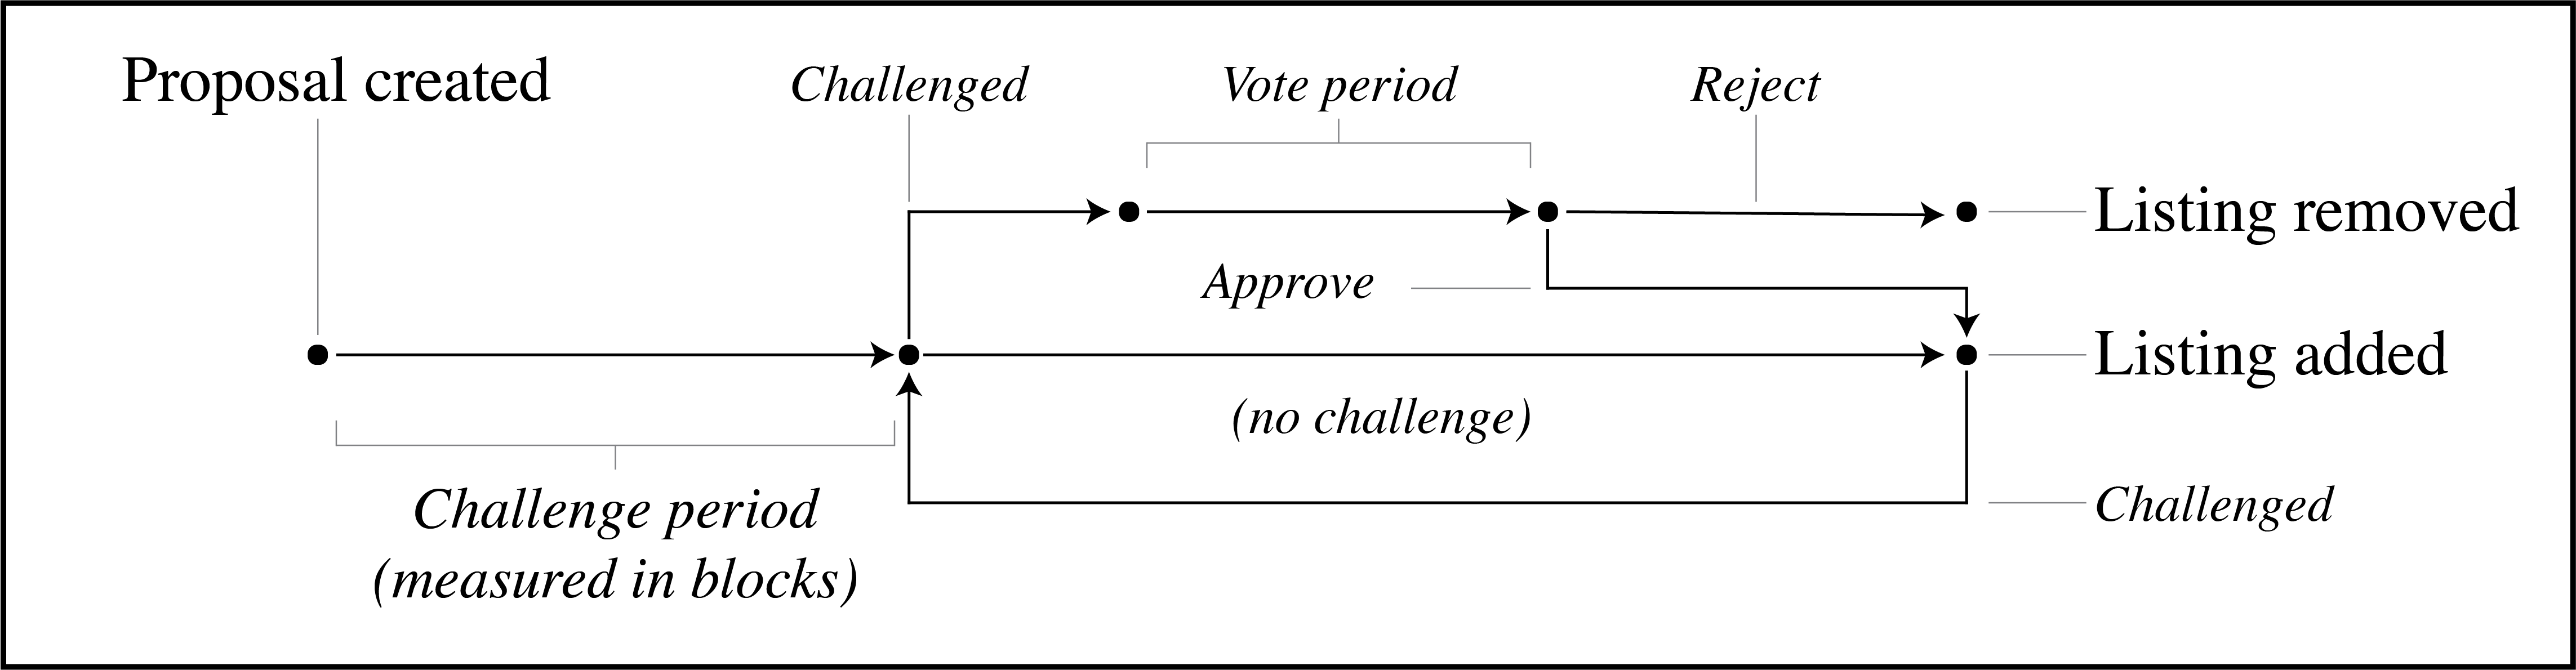
\includegraphics[width=\textwidth]{../figures/fig3.png}
  \caption{Simplified diagram of the Validator Registry listing curation cycle.}
  \label{fig:fig3}
\end{figure}

\begin{enumerate}
  \item Anyone may create a proposal that indicates their intent to become a network validator.
  \begin{enumerate}
    \item Proposals must include a stake greater than, or equal to a specified minimum stake.
    \item Proposals also include a ``reward'' to be executed to the validator on a periodic basis.
    \begin{enumerate}
      \item This reward may be positive (tokens minted), negative (tokens burned), or zero.
      \item If it is negative and the listing is accepted, the validator must continually collateralize a treasury balance sufficient to cover their burn rate.
      \item If they are unable to cover a burn, they may be removed from the listing without a full challenge (``touch-and-remove'').
      \item If a listing owners system balance falls below their stake size, they may also be touch-and-removed. 
    \end{enumerate}
    \item Proposals that are not challenged (see below) are automatically accepted after a period of time measured in Ethereum blocks.
  \end{enumerate}
  \item Pending proposals and accepted listings may be challenged at any time.
  \begin{enumerate}
    \item Challengers must have a system balance of tokens equal-to or greater-than the stake of the listing or proposal being challenged. 
    \item Challenges may be voted on by any Kosu token holder using a commit-reveal vote scheme during a specified voting period.
    \item Vote weight is determined by the balance of a user within the Kosu contract system.
    \item After the completion of a vote period, the ruling is determined based on the binary outcome that received a majority of the participating vote weight.
    \item If a challenge resolves against a listing or proposal, the listing's staked tokens are distributed to the challenger and the winning voters.
    \item If a challenge fails, the challenger's collateral is distributed to the winning voters and the owner of the challenged listing. 
    \item Voters are never penalized for voting on the losing side of a challenge.
    \item Failed challenges lose their collateral to the challenged listing and the winning voters.
  \end{enumerate}
\end{enumerate}
% END ETHEREUM CONTRACT SYSTEM SUB-SECTION
%%%%%%%%%%%%%%%%%%%%%%%%%%%%%%%%%%%%%%%%%%%%%%%%%%%%%%%%%%%%%%%%%%%%%%%%%%%%%%%%

%%%%%%%%%%%%%%%%%%%%%%%%%%%%%%%%%%%%%%%%%%%%%%%%%%%%%%%%%%%%%%%%%%%%%%%%%%%%%%%%
% BEGIN TENDERMINT NETWORK SUB-SECTION
\subsection{Tendermint Network}\label{tm-network}
\subsubsection{Introduction}\label{tm-network-intro}
The Kosu network is a Byzantine-Fault Tolerant (BFT) bonded proof-of-stake blockchain built on Tendermint Core that is designed to act as a decentralized order message aggregation and curation primitive\cite{bft, tendermint-wp}.
\medskip 

The core state machine, replicated across the network’s nodes by Tendermint, is designed with simplicity, efficiency, and safety in mind. It provides the minimal functionality necessary to establish a robust base layer upon which more sophisticated order booking and liquidity systems can be built.
\medskip

A primary feature of the network is the establishment of a canonical set of recent, valid  orders (see \ref{orders}) in each Kosu block. This order set, occasionally referred to as an ``order book'' due to helpful conceptual parallels, can be used to construct and verify a database of recent, curated order messages. This set of orders is computed deterministically by Kosu validators during block generation and transaction execution. A hash representing the canonical order set for each block is included in the application’s state tree (see section \ref{tm-network-state}).
\medskip

The network uses a shared security model, wherein Kosu validators are full Ethereum nodes, and thus must stay in sync with both chains. This model allows the Kosu network to maintain a one-way peg-zone with the Ethereum blockchain, where state changes to the Kosu contract system (balance updates, etc.) can be reflected in the Kosu network’s state, by way of special attestation ``witness'' transactions. Validators vote on and agree to apply state changes that receive support from a super-majority\footnote{\ Defined as { $ n \geq \frac{2}{3}$}, where {$n$} is an amount of vote power\cite{tendermint-wp}.} of the networks validating vote power.
\medskip

Order messages are treated as a finite network resource, constrained by physical bandwidth limitations, the number of transactions that can be included within a block, and the size of the order messages themselves. Order throughput is allocated to posters over discrete intervals called ``rebalance periods,'' which are parameterized by validators based on the height of the Ethereum blockchain, and a per-period order limit.
\medskip

Validators establish the maximum number of orders to accept per rebalance period as a configurable consensus parameter, and proportionally allocate throughput to posters based on the number of Kosu tokens each has bonded. This mechanic acts as a sybil tolerance mechanism, and creates a market for access to order throughput on the network. Individuals can always gain more bandwidth allocation by bonding more tokens in the Poster Registry (see \ref{ethereum-contract-system-poster-bonding}).
\medskip

Posters, individuals contributing order messages (see \ref{incentive-models}) to the network, sign their orders with the Ethereum keypair they used to bond tokens in the Poster Registry. When validators process these order transactions, the poster’s signature is recovered and checked against the in-state mapping of bandwidth allocations. Each valid order from a poster decrements their period limit by one, until a new period begins and the allocation is recomputed.
\subsubsection{Architecture}\label{tm-network-architecture}
Central to the Kosu protocol is its primary state application, a deterministic and finite transactional state machine, replicated across nodes by Tendermint Core and its underlying consensus engine. 
\medskip

The overall architecture of the Kosu network is similar to a conventional Tendermint network, with the addition of the infrastructure necessary to support a one-way peg-zone (see section \ref{peg}) to the Ethereum blockchain. The network is comprised of computing nodes running a client implementation of the Kosu network. Full nodes with Tendermint key-pairs that correspond to a listing in the Validator Registry (see \ref{ethereum-contract-system-tcr}) are designated as validators: they collect transactions and take turns proposing arrangements of the transactions in blocks, verifying the correct state changes have been made by comparing the Merkle root hash of the each new state. 
\medskip

The Kosu network’s architecture around a peg to the Ethereum blockchain is comparable to that of a side-chain, but there is an important distinction in that no state is shared from the Kosu network to the Ethereum contract system. The contract system is responsible for establishing the validator set and the poster account-balance mapping, and the network implements specific functionality based on this subsetted state. See section \ref{peg} for a full description of this one-way peg zone.
\medskip

The networks shared state is stored in Merkle tree that self-balances using a modification of the AVL algorithm, introduced by Tendermint\cite{tendermint-iavl}. Such a structure allows efficient verification about the correctness of a new state via the Merkle root after execution of a block (a requirement for consensus to be reached through Tendermint). Additionally, usage of a Merkle tree allows light-clients and applications to construct and verify proofs about the correctness of state contents.
\medskip

Kosu validators must run the following processes (some of which may be available through the same client implementation):

\begin{itemize}
  \item \underline{Ethereum client} - all validators must run full Ethereum nodes in order to track the Kosu contract system’s state, and to sign and submit necessary attestation transactions.
  \item \underline{Kosu state machine} - the primary application logic, which implements the Tendermint application blockchain interface (ABCI)\cite{tendermint-abci-spec}.
  \item \underline{Kosu Witness} - the validator process that maintains a connection to the Ethereum client, and implements the Kosu/Ethereum peg zone. Responsible for submitting Witness attestation transactions to the state machine.
  \item \underline{Tendermint Core} - manages peer-to-peer networking and state-machine replication of the Kosu sate machine via the Tendermint Consensus engine.
\end{itemize}

Validators likely will not run or provide public API or RPC services due to security concerns, therefore non-validating full-nodes play the important role of providing access to the network for most applications, infrastructure, and end users.
\medskip

Due to the fact that validators can be high-value targets for attacks (both for network denial-of-service, and targeted attacks to compromise the highly valuable validating keypairs), Kosu validators are expected to use special proxy full-nodes called ``sentries'' to access the network, and be isolated from the public internet\cite{sentry-architecture}.
\subsubsection{Poster access control}\label{tm-network-access}
The submission of order transactions is limited over deterministically calculated time intervals called rebalance periods. These periods are parameterized by validators with rebalance transactions (see \ref{tm-network-tx-types}) that specify the start and end of the period, indicated in Ethereum block heights. The rebalance periods additionally specify a maximum number of order transactions to accept within that period. 
\medskip

During the generation of these rebalance transactions, validators (via their Witness processes) snapshot the most up-to-date bonded balances of each account in the Poster Registry contract (see \ref{ethereum-contract-system-poster-bonding}), and proportionally allocate the number of orders to be accepted that period to posters based on the following equation.

\begin{equation}\label{bandwidth-equation}
  L_i =  P_{max} * \frac{B_i}{\sum_{i=1}^{n}B_i}
\end{equation}
\medskip

In equation \ref{bandwidth-equation} (above), $L_i$ represents the rate-limit of poster account $i$, $P_{max}$ is the total number of orders accepted per-period, $B_i$ is the bonded token balance of poster account $i$, and $n$ is the total number of poster accounts. This equation is parameterized and calculated at the beginning of each new rebalance period to generate the limit mapping for that period.
\medskip 

When the Ethereum block marking the end of a rebalance period is finalized\footnote{\ A block is considered finalized when it has reached a sufficient arbitrary age (number of blocks mined above it).}, each validator will create and sign a rebalance transaction, which includes a proposed rate-limit mapping constructed using the method described above. These transactions are verified based on the correct parameterization of the period (period length, order limit, etc.) as well as the accuracy of the proposed rate-limit mapping. 
\medskip

Rebalance transactions from non-Byzantine validators should include rate-limit proposals that match the one generated from existing in-state balances. Due to the fact that all rebalance transactions from behaving validators should be identical, it does not matter which proposal is accepted. The usual case is that the validator designated block proposer when the round-ending Ethereum block is finalized includes their own proposal. All subsequent proposals for that round will fail.
\medskip

As posters submit order messages (signed with their Ethereum keypair used to bond Kosu tokens), their per-period order limit is decremented until either it reaches zero and no more orders are accepted from that proposer, or a new period starts and their limit is re-computed and reset.
\subsubsection{State model}\label{tm-network-state}
Kosu nodes maintain an application state which includes the balance of poster accounts (updated through the peg-zone and witness mechanisms), the bandwidth allocation for posters (derived from their balance), information specific to the validator set to support its contract-based curation, and the parameterization of the active rebalance periods.
\medskip

The application's initial state is introduced in a hard-coded genesis block, and all subsequent states are generated deterministically from previous states and the transactions included within each block. Kosu’s genesis block will be generated after the contract system is deployed, allowing time for stakeholders to curate an initial validator set. Kosu’s genesis block will specify no initial validators. Instead, the genesis state generated from Kosu’s Ethereum contract system’s state at a specific height will reflect the staked balance of each entry in the Validator Registry, and the Kosu client implementation will deterministically generate and apply the genesis validator set during execution of the \texttt{InitChain} ABCI method upon initialization of the Kosu blockchain\cite{tendermint-abci-apps}.
\medskip

The state itself is represented in a mutable self-balancing AVL Merkle tree\cite{tendermint-iavl}, and the Merkle root hash is used to represent the \texttt{AppHash} included by Tendermint in the header of each block\cite{tendermint-abci-spec}.
\medskip

Usage of a Merkle tree data-structure enables proofs about the existence, absence, and correctness of state data, which is a necessity for a network such as Kosu that can benefit from the existence of light-clients (see section \ref{future-work}). It also enables the Kosu state machine to easily determine if it has the correct state for a new block by comparing the Merkle root hash of its own state against the \texttt{AppHash} included in each block’s header. Additionally, usage of an accurate and deterministic calculation, such as a Merkle root, allows Tendermint to safeguard the application from functioning in undefined states\cite{tendermint-abci-apps}. 
\medskip

Some of the notable structures maintained as part of the application's state are described below.

\bgroup
\def\arraystretch{1.2}
\begin{table}[H]
\centering
\label{table:table3}
\begin{tabularx}{1\textwidth}{|l|X|}
\hline
\textbf{Field name} & \textbf{Description} \\
\hline
\texttt{Posters} & A mapping of Ethereum addresses to poster accounts that contain a balance of staked tokens, and their current order limit (or quota) remaining for the active rebalance period. \\
\hline
\texttt{Validators} & A mapping of Tendermint-specific hashes of validator public keys (node IDs) to validator accounts that contain their associated Ethereum address, number of staked tokens, and fields used to track and record information about each validator. \\
\hline
\texttt{Events} & A mapping of Ethereum event data (identified by hashes of the data) populated from WitnessEvent transactions. Acts as a confirmation queue while events await sufficient confirmation from validator attestations. \\
\hline
\texttt{RebalanceInfo} & Stores the parameterization of the active rebalance period, including the starting and ending Ethereum heights, and the maximum number of orders to accept in the period. \\
\hline
\texttt{LatestOrders} & A fixed length, first-in-first-out hash list containing the transaction ID’s of a parameterizable number of the latest order transactions. This hash list makes up the stateful component of the network’s ``order book.'' \\
\hline
\end{tabularx}
\caption{Summary of important fields maintained in the network Merkle state trie.} 
\end{table}
\egroup

The primary account objects and state fields are described above, however other metadata fields are included in the state trie and ultimately affect the state’s Merkle root inserted in each Tendermint block header as the \texttt{AppHash}.
\subsubsection{Transaction types}\label{tm-network-tx-types}
The Kosu state machine implements four primary state-modifying transaction types, each described in detail in this section. Three of the transaction types are referred to as ``internal'' transactions, and require a signature from an active validator key-pair. These internal transactions (described below) facilitate the peg-zone to the Ethereum blockchain (see \ref{peg}) and manage access control for posters. 
\medskip

The fourth type of transaction are order transactions that require a signature from a valid poster account, and may be relayed (gossiped) to validators for inclusion in a block from full nodes. Internal transactions must only originate from validators.

\bgroup
\def\arraystretch{1.2}
\begin{table}[H]
\centering
\label{table:table4}
\begin{tabularx}{1\textwidth}{|l|l|X|}
\hline
\textbf{Message name} & \textbf{Internal} & \textbf{Description} \\
\hline
\texttt{WitnessEvent} & yes & Primary message type that supports the Ethereum peg zone. Submitted by each validator as an attestation to a state change to Kosu’s Ethereum contract system. Triggered by updates to poster’s bonded balances, and changes to the Validator Registry. \\
\hline
\texttt{WitnessRebalance} & yes & Submitted by validators at the end of each rebalance period to parameterize the next period. Includes a proposal for the poster rate-limit mapping which is verified against in-state balances. \\
\hline
\texttt{EthCheckpoint} & yes & Submitted by validators on a best-effort basis as an attestation to each new Ethereum block. Does not affect the rebalance mechanism or finality implementation, but can be used to verify correct age between finalized and new Ethereum blocks. \\
\hline
\texttt{ProposeOrder} & no & The only external (non-validator origin) transaction type, ProposeOrder messages are signed and submitted by bonded posters to add orders to the Kosu network. \\
\hline
\end{tabularx}
\caption{Summary of Kosu network's state-modifying transaction message types.} 
\end{table}
\egroup

\texttt{WitnessEvent} type transactions specify a ``subject'' field, which corresponds to the subject of the state change the event was generated to reflect. The subject can be set to ``posters'' for updates to the Poster Registry and the bonded balances of its accounts, or to ``validator'' for updates to the Validator Registry. WitnessEvents require a super-majority of active vote power to attest to a given event (identified by a deterministic hash) before the corresponding modification is made to the primary state, such as the addition or removal of a validator.
\medskip

\texttt{WitnessRebalance} transactions are submitted by validators when a rebalance period ends, marked by the maturation of the Ethereum block included in the period’s parameterization as the ending block. The submitted message includes a proposal for the poster rate-limit to be used in the next period. Because this mapping is generated deterministically from in-state balances, all WitnessRebalance proposals from non-Byzantine validators for a given period should be identical. Generally the rebalance transaction from the validator who happens to be proposing that block is accepted, given it matches the expected mapping from in-state balances. 
\medskip

\texttt{EthCheckpoint} transactions serve to correlate a given Kosu block height with the latest-known (non-matured) Ethereum block on a best-effort basis. Due to the possibility of reorganization of recent Ethereum blocks, the latest-known checkpoint is not used for any consensus critical mechanisms (such as generation of rate-limit mappings) and exists solely for validators to indicate the best-known Ethereum block. Validators submit an EthCheckpoint message each time a new Ethereum block is mined, and once a super-majority of validators attest to that block, it is accepted as the ``latest'' Ethereum block. 
\medskip

\texttt{ProposeOrder} transactions may be submitted by posters who have bonded Kosu tokens in the Poster Registry, and count against that poster’s rate-limit for the active rebalance period. Assuming the ProposeOrder message is structurally valid, and the signature is recoverable and originated from a poster account with a remaining limit, the order is accepted. Upon acceptance of an order, the posters limit is decremented, and the order’s hash is added to a fixed-length first-in-first-out order hash list included in the network’s Merkle root.
\subsubsection{Validator curation}\label{tm-network-validators}
A motivating requirement of Kosu’s design was the ability to support a highly dynamic proof-of-stake validator set. The incentive model of the overall protocol (see \ref{incentive-models}) requires that protocol stakeholders have the ability to curate the networks validators, both to facilitate healthy competition for the position, and to allow the removal of validators who may not be explicitly byzantine (by lying or attempting to compromise consensus), but who may otherwise be engaging in behavior stakeholders deem implicitly malicious. These considerations motivated the design of the curation mechanism (described in section \ref{ethereum-contract-system-tcr}) and supporting peg-zone (described in \ref{peg}).
\medskip

Kosu’s underlying networking and consensus engine, Tendermint Core, allows a genesis validator set to be hard-coded or computed during network genesis, and for updates to the validator set to be applied by existing validators at the end of each block\cite{tendermint-abci-apps}.
\medskip

To avoid the special case of selecting genesis validators to launch the network with, the Kosu protocol’s launch will be multi-phased, with the contract system being deployed ahead of the networks genesis. Deploying the contract system prior to the launch of the network will allow the decentralized curation mechanism to produce an initial listing state, which can be used to compute the initial validator set. 
\medskip

A specific Ethereum block height will be agreed upon at which point node operators will snapshot the contract system’s state, and populate Tendermint’s genesis file with the initial state. During the one-time execution of the \texttt{InitChain} ABCI method \cite{tendermint-abci-apps}, the Kosu state application will apply the deterministically-computed genesis validator set and block production will begin. All listings included in the registry at the specified Ethereum block will become the network’s first validators, from which point normal network operation and peg-zone functionality will commence.
\medskip

The next section introduces the Kosu Ethereum peg-zone, and provides an overview of its construction and implementation.
% END TENDERMINT NETWORK SUB-SECTION
%%%%%%%%%%%%%%%%%%%%%%%%%%%%%%%%%%%%%%%%%%%%%%%%%%%%%%%%%%%%%%%%%%%%%%%%%%%%%%%%

%%%%%%%%%%%%%%%%%%%%%%%%%%%%%%%%%%%%%%%%%%%%%%%%%%%%%%%%%%%%%%%%%%%%%%%%%%%%%%%%
% BEGIN PEG NETWORK SUB-SECTION
\subsection{Ethereum Peg Zone}\label{peg}
\subsubsection{Introduction}\label{peg-intro}
Communication between blockchains, specifically those with differing types of finality guarantees, requires the usage of a peg-zone. The Ethereum blockchain currently offers probabilistic finality for state-modifying transactions included in blocks based on its proof-of-work consensus mechanism. Older PoW blocks are exponentially harder to reorganize than recently mined blocks, thus as the age of a block increases, the chance of that block or its contents being moved in the blockchains chronology decreases exponentially\cite{blockchain-taxonomy}.
\medskip

This is in contrast to the security model Kosu uses where economic finality is guaranteed nearly instantly, thanks to the underlying Tendermint Consensus engine\cite{tendermint, tendermint-wp}. As soon as a super-majority of the network’s vote power supports the commit of a given block, it can be considered finalized and irreversible. It would be impossible for any entity to ``reorganize'' the canonical chain in the proof-of- work sense without possessing a super-majority of vote power through the acquisition of a significant number of 
Kosu tokens, and approval to the validator set by existing token holders.
\medskip

The Kosu to Ethereum one-way peg-zone facilitates a small subset of Ethereum’s state to be represented on the Tendermint-based network. The usage of a one-way peg allows Kosu to leverage the security and uptime of the Ethereum network for critical extra-protocol actions, such as the transfer and exchange of KOSU tokens, and validator set curation.
\medskip

Generalized and two-way peg-zones require complex construction\cite{peggy-spec} and additional security assumptions, so Kosu uses a simple architecture for its peg-zone that is specific to a subset of state changes in the Kosu contract system (see \ref{ethereum-contract-system}).
\subsubsection{Architecture}\label{peg-architecture}
The architecture and design of Kosu’s one-way peg-zone is conceptually simple, and builds off a two-way peg-zone design initially proposed by Cosmos\cite{peggy-spec}. Kosu’s peg zone comprises of two main components, one residing in the Kosu contract system, and the other as part of Kosu’s Tendermint-based network.
\medskip

Kosu’s contract system (see \ref{ethereum-contract-system}) contains a special ``logging'' contract called the EventEmitter which emits descriptive event logs for certain state changes to the overall contract system. The Kosu peg-zone implementation is concerned with two types of events emitted by the EventEmitter.
\medskip

One event type describes an update to the Poster Registry, when a new poster bonds token, or an existing poster modifies their balance by adding or withdrawing tokens. The event contains the Ethereum address of the poster, and an unsigned integer representing their new balance (which may be zero).
\medskip 

The second event describes updates to the ValidatorRegistry, when a new validator is added, or an existing validator is removed. The event contains the Ethereum address to be associated with the validator, the number of Kosu tokens they have put at stake (which directly affects network vote power), as well a 32-byte ED25519 public key to be registered as a validating key\cite{tendermint-crypto-spec}. See section \ref{ethereum-contract-system-tcr} for a description registries logic. For the purposes of the peg-zone, all that matters is an event is emitted with each change to the registry’s state.
\medskip

The peg-zone is implemented as part of the Kosu network by a special process validators run called a Witness. All validators are required to run full Ethereum nodes, and submit attestation transactions for each of the pertinent events (described above, and in detail below), signed with their validating key pair. 
\medskip

When a super-majority of active validators\footnote{\ Measured in terms of vote power, the number of validators does not matter.} submit attestation transactions to the Kosu network about a given event from the contract system, that event is ``applied'' to the network’s state by updating the necessary account in the case of a poster, or by applying a modification to the validator set.
\subsubsection{Process description}\label{peg-process}
\begin{figure}[H]
  \centering
  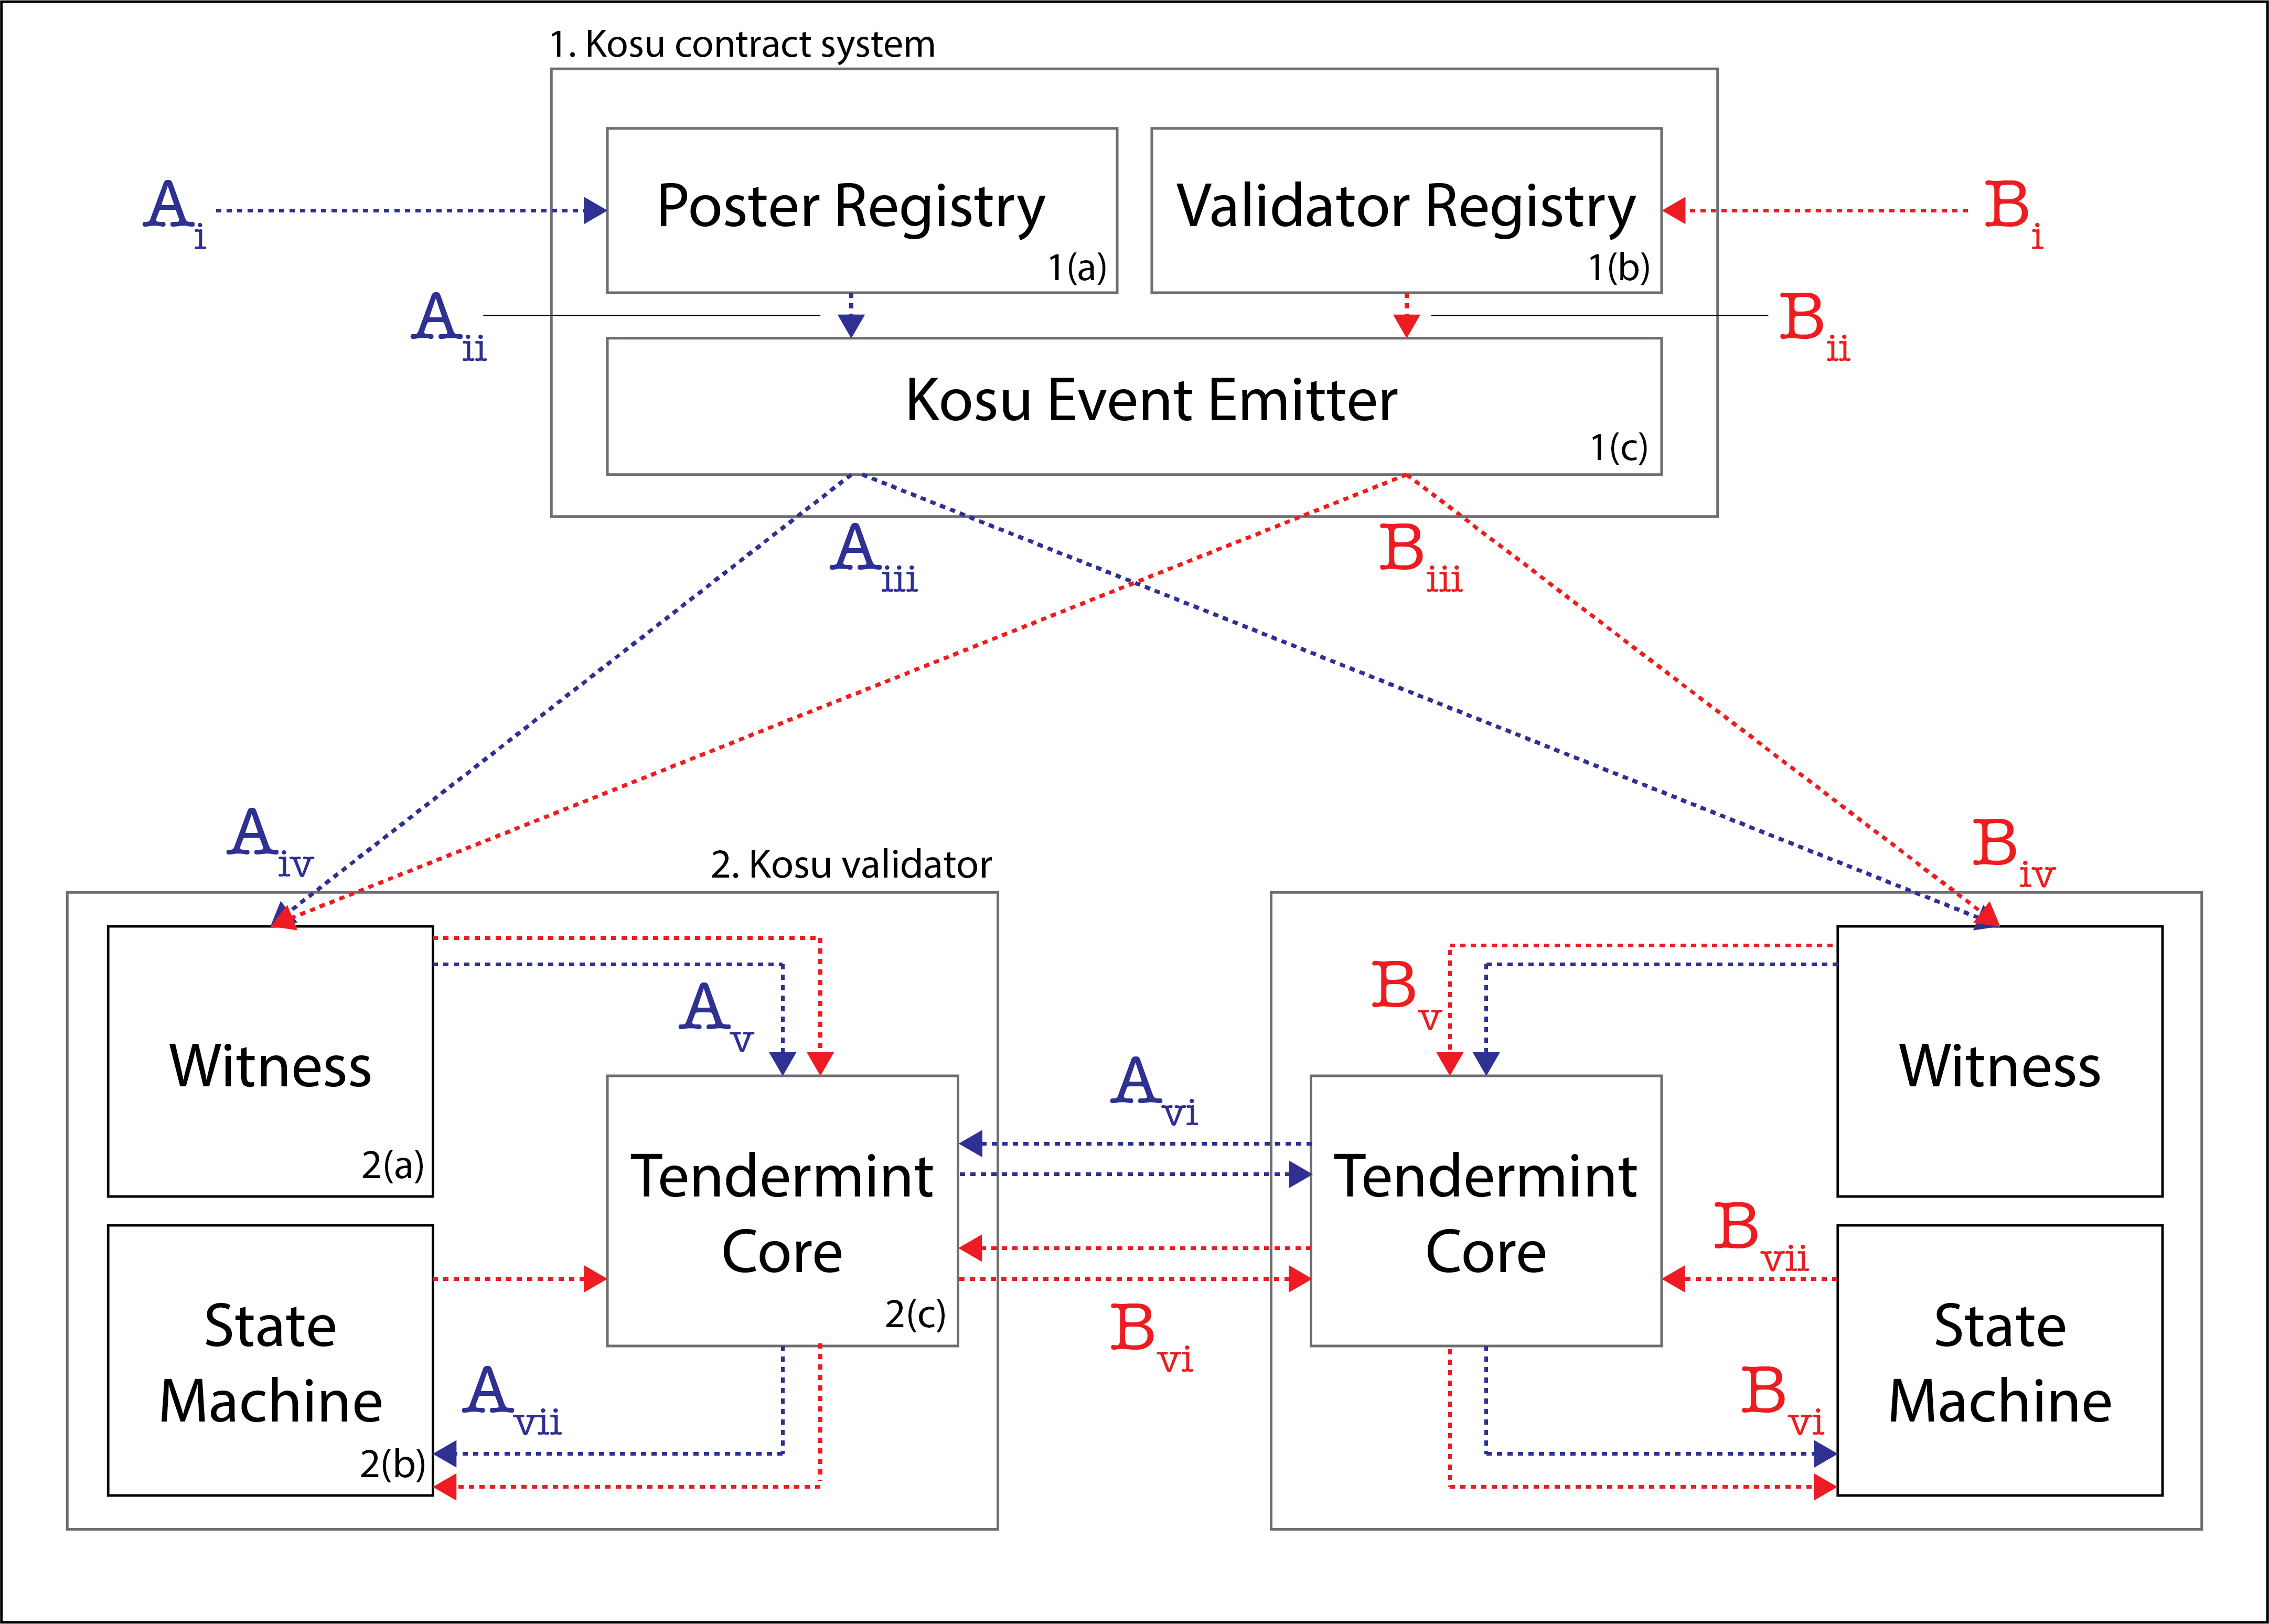
\includegraphics[width=\textwidth]{../figures/fig1.png}
  \caption{A simplified diagram of the systems involved in the Kosu-Ethereum peg zone. Box 1 shows components of the Kosu contract system, box 2 shows components of Kosu validators. The processes illustrated in red and blue are described below.}
  \label{fig:fig2}
\end{figure}

Below is a simplified description of the processes involved in updating a poster account (A, solid lines in fig. \ref{fig:fig2}) or modifying the validator set (B, dashed lines in fig. \ref{fig:fig2}) as part of normal peg-zone functionality. The diagram shows only two validators for illustrative purposes, a live network should never operate with less than four validators, the minimum required to tolerate a single fault (Byzantine or otherwise).
\medskip

The process of updating the network’s validator set and poster accounts is similar, as both use the same witness infrastructure. However, there are important distinctions between how the events are initially generated, and the transitions they effect within the underlying Kosu state machine.

\begin{enumerate}[A.]
  \item Addition, removal, or modification of a poster account (shown as A, solid lines in fig. \ref{fig:fig2}):
  \begin{enumerate}[i.]
    \item A poster entity submits a bond or unbond transaction to the PosterRegistry.
    \item If the transaction is valid, it is included in an Ethereum block and the registry calls a function on the EventEmitter contract during execution of the transaction.
    \item The EventEmitter contract produces an event log containing the posters address, their new balance, and additional meta-data.
    \item The Witness process on active validators is notified of the event from a local Ethereum node. After a certain confirmation threshold (measured in Ethereum blocks) passes, the Witness will sign a Kosu WitnessTransaction with the validators keypair attesting to the event.
    \item The validator’s attestation is submitted to their local Tendermint instance.
    \item Tendermint propagates the attestations throughout the network to be validated, executed, and ultimately to be included in a block.
    \item When the transactions reach the underlying state machine, they are added to a confirmation queue where they await sufficient confirmation from a super-majority of validating vote power. Once the confirmation threshold reached, the state change is applied to the necessary poster account to reflect their updated balance of bonded Kosu tokens.
  \end{enumerate}
  \item Addition or removal of a Kosu validator (shown as B, dotted lines in fig. \ref{fig:fig2}):
  \begin{enumerate}[i.]
    \item A validator listing is confirmed into (or voted out of) the ValidatorRegistry (exact process detailed in section \ref{ethereum-contract-system-tcr})
    \item During execution of an Ethereum transaction that confirms the validator’s listing update, a function call is made to the EventEmitter contract.
    \item The EventEmitter contract produces an event with the validator’s Ethereum address, their Tendermint public key, and their staked balance (which is set to zero in the case of a removal).
    \item A validator’s active Witness process receives and parses the event, and waits for the necessary number of Ethereum blocks to be mined above the block the event-trigger transaction was included in.
    \item The validator’s Witness component signs a Kosu WitnessEvent transaction attesting to the update, and submits it to the network via Tendermint.
    \item Tendermint propagates the attestation to other validators for inclusion in an upcoming block. 
    \item Similar to poster events, new attestations are added to a confirmation queue until sufficient attestations are received about the event from active validators.
    \item At this point, the process differs from the handling of poster balance updates. When the validator update event is confirmed, existing validators include a set of fields in the \texttt{EndBlock} response message sent to Tendermint that indicates the adjustment to the validator set. In the case of a new validator, the new public key is assigned a vote weight equal to the number of staked tokens\footnote{\ A conversion factor is required to avoid integer overflow of the Tendermint vote power representation.}. If the validator is removed, their vote power is set to zero. The update applied at block \texttt{H} takes enables a new validator to join the set and participate in consensus, starting at block \texttt{H+2}\cite{tendermint-abci-spec}.
  \end{enumerate} 
\end{enumerate}
% END PEG SUB-SECTION
%%%%%%%%%%%%%%%%%%%%%%%%%%%%%%%%%%%%%%%%%%%%%%%%%%%%%%%%%%%%%%%%%%%%%%%%%%%%%%%%

%%%%%%%%%%%%%%%%%%%%%%%%%%%%%%%%%%%%%%%%%%%%%%%%%%%%%%%%%%%%%%%%%%%%%%%%%%%%%%%%
% BEGIN INCENTIVE MODEL SUB-SECTION
\subsection{Incentive Models}\label{incentive-models}

\subsubsection{Validators}\label{incentive-models-validators}
The network described above utilizes a bonded proof-of-stake system to manage sybil tolerance. Validators are required to make a security deposit, also known as a stake, in order to participate in consensus. Tendermint Consensus allows certain types of malicious behavior committed by validators to be easily verified and punished accordingly. 
\medskip

The KOSU network makes a few core assumptions that influence the design of the validator incentive model. Such assumptions are motivated below.

\begin{enumerate}[I.]
  \item Validators are expected to capture both explicit and implicit rewards.
  \begin{itemize}
    \item Central topographical positioning within the network provides validators with unique informational asymmetries that can be exploited for profit.
    \item Discouraging such behavior without obscuring transactional information is not immediately desirable.
  \end{itemize}
  \item Implicit reward capture is highly variable and progressive.
  \begin{itemize}
    \item There exists a direct relationship between network usage and the frequency of exploitable information.
    \item Though the value of the informational asymmetries provided to validators is not easily quantifiable, we can expect there exists a positive correlation between network usage and the value of implicit reward capture.
  \end{itemize}
  \item The number of validators is negatively correlated with network performance.
  \begin{itemize}
    \item Network security is a function of both the distribution of wealth as well as the total bonded token quantity of validators.
    \item Comparatively (and in a controlled setting), network performance is purely a function of validator quantity.
    \item As more validators are added to the network, latency increases absolutely.
  \end{itemize}
\end{enumerate}

These assumptions motivate a market driven fee schedule for a validator set that is dynamic in both size and inclusion. The ValidatorRegistry system (described in section \ref{ethereum-contract-system-tcr}) allows for exactly this. To become a validator, a candidate must bond an unspecified amount tokens (above the parameterizable minimum), which will provide them a proportional influence in consensus, as well as define a requested fee schedule. The expected economic impact of a proposal (via inflation, security, latency) motivates a focal point on a continuum that will eventually resolve in a binary direction.
\medskip

It is important to note that this validator selection model is considerably more subjective than largest-bond (rank) based proof-of-stake validator selection mechanisms. With that said, the unique domain requirements as well as the limited impact of malicious validator behavior seem to warrant such subjectivity.
\medskip

The listing can be challenged at any time by submitting a challenge proposal with a stake equivalent to the stake of the bonded validator. If the challenge succeeds, the validator is removed from the registry and loses their stake, which is distributed to voters on the winning outcome proportionally to token weight with extra reward given to the challenge initiator. This challenge method is a stakeholder-based slashing mechanism that is designed to regulate subjectively malicious value capture behavior.
\medskip

More explicit byzantine behaviors can be enforced structurally via explicit slashing conditions based on fraud/liveness proofs. Conditions/behaviors that could be discouraged explicitly include double voting, low validator liveness, incorrect event witnessing etc.

\subsubsection{Posters}\label{incentive-models-posters}
In order to regulate network spam, posters, individuals contributing order data to the network, are required to bond tokens. Posters are awarded network access in the form of order bandwidth allocation proportional to their bonded token quantity. In this model, the inclusion of transactions is not fee based, but rather bandwidth based. This is a significant design feature of the network motivated on the basis that quality liquidity creation should be rewarded, and transaction fees are not compatible in this regard. Individual orders are not necessarily valuable, thus network contributions should be feeless so long as the contributor’s incentives are aligned with those of the greater network.
\medskip

Unlike validators, the behavior of posters is not directly punishable via slashing. Instead, the poster bond is intended to implicitly align the economic incentives of posters with the success of the overall network and create sybil tolerance via token scarcity. As the usage of the network increases, posters contributing quality orders are rewarded via token appreciation. Conversely, there is an economic disincentive for posters to post spam as this would result in a depreciated token value.
\medskip

In this model, there does exist the potential for ``free-riders,'' particularly speculators benefiting from the appreciation of KOSU value as a result of liquidity providers’ work. While not completely ideal, this artifact is not entirely corrupt as the ``free-riders'' do in fact contribute to the security of the protocol by increasing token scarcity. 

\subsubsection{Voters}\label{incentive-models-voters}
The validator selection model used by the Kosu network is relatively subjective, requiring the active participation of token holders in the curation of a validator set. Due to the magnitude of such decisions, it is important to maximally incentivize participation via explicit participation rewards. 
\medskip

Token holders participating in the curation mechanisms, including those who submit winning challenges and vote correctly in challenges earn KOSU tokens as rewards. This results in an active token distribution directed towards participating and benevolent network actors. It is important to note that all token holders, including those bonded as both validators and stakers, can participate in any election/decision.
% END INCENTIVE MODEL SUB-SECTION
%%%%%%%%%%%%%%%%%%%%%%%%%%%%%%%%%%%%%%%%%%%%%%%%%%%%%%%%%%%%%%%%%%%%%%%%%%%%%%%%

\clearpage
\pagebreak
% END SPECIFICATION SECTION

%%%%%%%%%%%%%%%%%%%%%%%%%%%%%%%%%%%%%%%%%%%%%%%%%%%%%%%%%%%%%%%%%%%%%%%%%%%%%%%%
%~~~~~~~~~~~~~~~~~~~~~~~~~~~~~~~~~~~~~~~~~~~~~~~~~~~~~~~~~~~~~~~~~~~~~~~~~~~~~~%
%%%%%%%%%%%%%%%%%%%%%%%%%%%%%%%%%%%%%%%%%%%%%%%%%%%%%%%%%%%%%%%%%%%%%%%%%%%%%%%%

% BEGIN TOKEN DISTRIBUTION SECTION
\section{Token Distribution}\label{token-distribution}

\subsection{Overview}\label{token-distribution-overview}
Token distribution is a key determinant of incentive compatibility for the models defined previously. Kosu’s proposed token includes multiple utilities that collectively catalyze wealth distribution to be a relatively dynamic process. To complement such dynamism, Paradigm Labs plans a continuous token distribution via a market-driven, validator defined reward system (outlined previously) and a bonding curve. KOSU’s distribution will thus be a function of both a determinant process, the bonding curve, and an indeterminate process, the validator reward schedule.
\medskip

Preceding an official network launch, a contract responsible for token distribution will be deployed\footnote{To preserve fairness, no tokens will be pre-mined. With that said, the bonding functions will be exponential in order to incentivize early participation.}. The contract will be permissioned to mint additional KOSU tokens based on an algorithmic pricing model. It will allow users to receive KOSU by bonding Ether (ETH) and vise versa. The pricing model defines a parametric equation that allows bonding curves to be dynamically defined based on the existing token contract state. This construction maintains the correctness of the system by providing an additional independent variable necessary for price adjustment due to token inflation as a result of validator rewards.

\subsection{Mechanics}\label{token-distribution-mechanics}
In order to gain intuition about the system and parametric equation used, we will consider the following derivation.
\medskip

Let us define a slightly exponential family of curves $ y = m*x^n $ where $y$ is the price of KOSU denominated in ETH, $x$ is the KOSU supply, $n$ is a predetermined constant within the range $(1,2)$ and $m$ is the slope which is parameterized upon each bond/unbond transaction. The power function $y$ represents the price of KOSU denominated in ETH and $x$ defines the total KOSU supply. We can thus calculate the total amount paid, which should correspond to the total pool balance $b$, at some token supply $j$ with the following integral calculation.

\begin{equation}\label{full-bonding-integral}
  b = \int_{0}^{j} m*x^n dx = \frac{m}{n+1}j^{n+1}
\end{equation}
\medskip

\noindent Solving for $m$: 

\begin{equation}
  m = \frac{b(n+1)}{j^{n+1}}
\end{equation}
\medskip

Borrowing from Bancor, let us now define a constant called the reserve ratio, $r$, which gives the quotient of the current pool balance and the product of the token supply, $j$ and the price at this point, $p_j$\cite{bancor-whitepaper}.

\begin{equation}\label{reserve-ratio}
  r = \frac{b}{p_j*j}
\end{equation}
\medskip

\noindent From equations \ref{full-bonding-integral} and \ref{reserve-ratio}, we get:

\begin{equation}
  r = \frac{\frac{m}{n+1}j^{n+1}}{j*(m*j^n)} = \frac{1}{n+1}
\end{equation}
\medskip

\noindent From which we can calculate:

\begin{equation}
  n = \frac{1}{r}-1
\end{equation}
\medskip

\noindent Substituting our newly derived representations of $m$ and $n$ and simplifying, we can derive the following parametric equation.

\begin{equation}\label{parametric-eq}
  y = \frac{b}{r*j^{\frac{1}{r}}}*x^{\frac{1}{r}-1}
\end{equation}

Where (in equation \ref{parametric-eq}) $y$ is the KOSU price denominated in Ether, $x$ is the quantity of KOSU bonded, $j$ is the total KOSU supply, $b$ is the total quantity of Ether collateral (pool balance), and $r$ is the reserve ratio, defined in equation \ref{reserve-ratio}.
\medskip 

From equation \ref{parametric-eq}, we can further derive equations for calculating payouts in both directions. The equation for both payout directions are included below. For a more formal derivation of the equations referenced below, please refer to Bancor’s ``Formulas for Bancor system''\cite{bancor-formulas}. 
\subsection{Ether to Kosu}\label{token-distribution-eth-kosu}
\begin{equation}
  \beta = j* ((\frac{1+\alpha}{b})^{\frac{b}{p*j}} - 1)
\end{equation}
\medskip

Where $\alpha$ is the quantity of Ether deposited, $\beta$ is the quantity of KOSU received, $j$ is the current KOSU supply, $b$ is the quantity of Ether collateral (pool balance), and $p$ is the price of KOSU (in Ether) at supply level $j$. 
\subsection{Kosu to Ether}\label{token-distribution-kosu-eth}
\begin{equation}
  \alpha = b* ((\frac{1+\beta}{j})^{\frac{p*j}{b}} - 1)
\end{equation}
\medskip

Where $\beta$ is the quantity of KOSU deposited, $\alpha$ is the quantity of Ether received, $j$ is the current KOSU supply, $b$ is the quantity of Ether collateral (pool balance), and $p$ is the price of KOSU (in Ether) at supply level $j$. 
\clearpage
\pagebreak
% END TOKEN DISTRIBUTION SECTION

%%%%%%%%%%%%%%%%%%%%%%%%%%%%%%%%%%%%%%%%%%%%%%%%%%%%%%%%%%%%%%%%%%%%%%%%%%%%%%%%
%~~~~~~~~~~~~~~~~~~~~~~~~~~~~~~~~~~~~~~~~~~~~~~~~~~~~~~~~~~~~~~~~~~~~~~~~~~~~~~%
%%%%%%%%%%%%%%%%%%%%%%%%%%%%%%%%%%%%%%%%%%%%%%%%%%%%%%%%%%%%%%%%%%%%%%%%%%%%%%%%

% BEGIN FUTURE WORK SECTION
\section{The Matcher Model}\label{matcher-model}
There will inevitably exist a wide distribution in the technical sophistication of Kosu users. Traders, for example, may have little understanding of the bonding concept used by the system to maintain access control. Other subtleties, including issues with order collisions and front running, should not be assumed knowledge for general users of the system. As such, second-layer services should provide abstractions of the system’s many complexities. In addition to improving user experience, these abstractions concentrate the network's stakeholders to a more participatory group.
\medskip 

For makers, these services might provide an endpoint with an associated quantity of bonded tokens, allowing users to post limit orders through an GUI/API without needing to bond tokens themselves. These could be structured as free services (entities hold KUSO tokens and expect their liquidity contribution to accrue value via the appreciation of the underlying token) or for a per-post fee.
\medskip

For servicing takers, these second-layer systems may function similarly to designated market makers in dealers markets; providing direct liquidity with quotes adjusted by a premium for the assumed execution risk.
\clearpage
\pagebreak
% END FUTURE WORK SECTION

%%%%%%%%%%%%%%%%%%%%%%%%%%%%%%%%%%%%%%%%%%%%%%%%%%%%%%%%%%%%%%%%%%%%%%%%%%%%%%%%
%~~~~~~~~~~~~~~~~~~~~~~~~~~~~~~~~~~~~~~~~~~~~~~~~~~~~~~~~~~~~~~~~~~~~~~~~~~~~~~%
%%%%%%%%%%%%%%%%%%%%%%%%%%%%%%%%%%%%%%%%%%%%%%%%%%%%%%%%%%%%%%%%%%%%%%%%%%%%%%%%

% BEGIN FUTURE WORK SECTION
\section{Future Work}\label{future-work}
\subsection{Formalized Governance}\label{future-work-governance}
A special privilege afforded to the core development team will be the responsibility of managing specific system parameters. These parameters include total bandwidth, the exponential rate of the token bonding curve, finality threshold, etc.
\medskip

At genesis and for the foreseeable future, the management of these parameters will be at the discretion of the Paradigm Labs team who intend to publicly involve significant stakeholders in an informal collective decision making process. 
\medskip

Paradigm Labs intends to eventually transition such control to a more formal decentralized governance system, following cues from well-established protocol’s that are also pursuing similar systems.

\subsection{Decentralized Trade Execution}\label{future-work-tec}
Orders shared on the Kosu network are (generally) public in the sense that any taker can become a counterparty by submitting the signed order message to the layer-one network and settlement contract system specified by the order. With account based layer one networks like Ethereum, these transactions are batched into blocks. In the scenario where multiple parties attempt to fill an order, the order that is included first will settle while the other will fail. This means that the taker whose transaction failed will waste gas and effort.
\medskip

The 0x project has proposed various solutions to this problem including the introduction of a Trade Execution Coordinator which can enforce execution scenes such as price time priority and selective delay off-chain via specific order construction and a contract extension\cite{0x-selective-delay}.
\medskip

The current implementation of the TEC system proposed by 0x is not trustless, but is expected to evolve towards a decentralized solution\cite{0x-coordinator-specification}. This work is particularly important for competitive/liquid markets as it will contribute to reduced spreads by reducing front-running opportunities. Kosu is designed to be agnostic to execution systems and will thus benefit from any progress made at this layer.

\subsection{Decentralized Price Oracles}\label{future-work-oracles}
Secure and scalable decentralized price oracles are a juggernaut. Many projects within the decentralized finance space currently require trusted price feeds that provide little accountability for correctness. This is a large hole within the decentralization of many existing protocol architectures.
\medskip

Recently, the Marble team released Polaris, an on-chain decentralized price oracle for ERC20 tokens. Polaris works by calculating the median of historical checkpoints on Uniswap\cite{polaris-intro-article}. Polaris is a step in the correct direction, but will be fundamentally limited in security by the adoption of the underlying exchange primitive, Uniswap. Uniswap provides a compelling automated market making solution for decentralized exchange, but requires active arbitrageurs for price convergence. This means Uniswap’s system is effectively price discovery by arbitrage. In our team’s opinion, the scalability potential of this solution is limited\cite{uniswap-docs}. As such, we believe the best way to scale a decentralized price oracle is likely off-chain. 
\medskip

There are a few viable approaches to this problem. Perhaps a medianized rate, as determined by a curated set of participants, is sufficient for some applications. However, we believe that a strong decentralized price oracle should enforce price calculation in an explicit and auditable manner. To do so, requires a consistent set of valid orders, as well as guarantees around the public visibility and fillability of such orders. Though complex in construction, Kuso might provide the basis for such a system. Kuso maintains checkpoints to the Ethereum chain and provides strong consistency for a globally maintained order set. Together, these properties could potentially be leveraged to create proofs of validity, visibility and ultimately price. 
\medskip

With that said, the strength of such a system, as referenced in the Uniswap discussion, is heavily dependent on adoption of the underlying protocol. The viability of such a system is also heavily dependent on minutiae regarding implementation. Nevertheless, the possibility of such a system is intriguing.
\clearpage
\pagebreak
% END FUTURE WORK SECTION

%%%%%%%%%%%%%%%%%%%%%%%%%%%%%%%%%%%%%%%%%%%%%%%%%%%%%%%%%%%%%%%%%%%%%%%%%%%%%%%%
%~~~~~~~~~~~~~~~~~~~~~~~~~~~~~~~~~~~~~~~~~~~~~~~~~~~~~~~~~~~~~~~~~~~~~~~~~~~~~~%
%%%%%%%%%%%%%%%%%%%%%%%%%%%%%%%%%%%%%%%%%%%%%%%%%%%%%%%%%%%%%%%%%%%%%%%%%%%%%%%%

% BEGIN BIBLIOGRAPHY
\begin{thebibliography}{9}

\bibitem{tendermint}
All In Bits Inc., Tendermint, et al. ``Tendermint Consensus Reactor.''
\\\texttt{https://bit.ly/tendermint-consensus-reactor}

\bibitem{0x-coordinator-specification}
Bandeali, Amir and Berger, Fabio. ``0x 2.0.0 Coordinator Specification.''
\\\texttt{https://bit.ly/0x-coordinator-spec}

\bibitem{0x-roadmap-pt-2}
Bloemen, Remco. ``0x Roadmap 2019 (part 2): Scalability R\&D.''
\\\texttt{https://bit.ly/0x-scalability-pt-2}

\bibitem{tendermint-abci-apps}
Buchman, Ethan., et al. ``Application Blockchain Interface Specification (Applications).''
\\\texttt{https://bit.ly/tendermint-abci-applications}

\bibitem{tendermint-abci-spec}
Buchman, Ethan., et al. ``Application Blockchain Interface Specification (Methods and Types).''
\\\texttt{https://bit.ly/tendermint-abci-spec}

\bibitem{tendermint-iavl}
Buchman, Ethan., et al. ``Merkleized IAVL+ Tree implementation in Go''
\\\texttt{http://bit.ly/tendermint-iavl}

\bibitem{tendermint-crypto-spec}
Buchman, Ethan., et al. ``Tendermint Core specification: Encoding and Digests.''
\\\texttt{https://bit.ly/tendermint-encoding-spec}

\bibitem{ethereum-whitepaper}
Buterin, Vitalik., et al. ``Ethereum White Paper.''
\\\texttt{https://bit.ly/ethereum-white-paper}

\bibitem{flash-boys-2}
Daian, Philip., et al. ``Flash Boys 2.0: Frontrunning, Transaction Reordering, and Consensus Instability in Decentralized Exchanges.''
\\\texttt{https://bit.ly/flash-boys-paper}

\bibitem{tendermint-wp}
Ethan Buchman, et al. ``Tendermint: Byzantine Fault Tolerance in the Age of Blockchains.''
\\\texttt{https://bit.ly/tendermint-thesis}

\bibitem{kosu-sdk}
Freyaldenhoven, Nick., et al. ``Kosu SubContract SDK.''
\\\texttt{https://bit.ly/kosu-settlement-sdk}

\bibitem{tcr-1}
Goldin, Michael. ``Token Curated Registries 1.0.'' Medium.
\\\texttt{https://bit.ly/token-curated-registries}

\bibitem{bancor-whitepaper}
Hertzog,  Eyal., et al. ``Bancor Protocol: Continuous Liquidity for Cryptographic Tokens through their Smart Contracts.''
\\\texttt{https://bit.ly/bancor-white-paper}

\bibitem{dharma-wp}
Hollander, Nadav. ``Dharma: A Generic Protocol for Tokenized Debt Issuance.''
\\\texttt{https://bit.ly/dharma-whitepaper}

\bibitem{peggy-spec}
Kunze, Federico, et al. ``Two-way Permissionless Peg Zones.'' Tendermint.
\\\texttt{https://bit.ly/peggy-spec}

\bibitem{bft}
Leslie Lamport, Robert Shostak, Marshall Pease. ``The Byzantine Generals Problem.''
\\ACM Transactions on Programming Languages and Systems, Vol. 4, No. 3. July 1982. Pages 382-401.

\bibitem{capital-markets-report}
McKinsey Global Institute, ``\$118 Trillion and Counting: Taking Stock of the World's Capital Markets.''
\\\texttt{https://bit.ly/mckinsey-capital-report}

\bibitem{kosu-monorepo}
Paradigm Labs, corp., et al. ``Kosu Monorepo: A Monorepo for the Kosu Protocol.''
\\\texttt{https://bit.ly/kosu-protocol-repo}

\bibitem{paradigm-github}
Paradigm Labs, corp., et al. ``Paradigm Labs GitHub.''
\\\texttt{https://bit.ly/paradigm-labs-github}

\bibitem{polaris-intro-article}
Pereira, Mykel. ``Introducing Polaris: A trustless price oracle for ERC20 tokens on Ethereum Mainnet.''
\\\texttt{https://bit.ly/polaris-intro}

\bibitem{sentry-architecture}
Ramsay, Zack., et al. ``Tendermint Core specification: Peer Discovery''
\\\texttt{https://bit.ly/tendermint-node-spec}

\bibitem{bancor-formulas}
Rosenfeld, Meni. ``Formulas for Bancor system.''
\\\texttt{https://bit.ly/bancor-formulas}

\bibitem{blockchain-taxonomy}
Tasca, Paola., Tessone, Claudio. J. ``Taxonomy of Blockchain Technologies; Principles of Identification and Classification.''
\\\texttt{https://bit.ly/taxonomy-of-blockchains}

\bibitem{uniswap-docs}
Uniswap. ``Uniswap Exchange Protocol Documentation.''
\\\texttt{https://bit.ly/uniswap-docs}

\bibitem{erc-20}
Vogelsteller, Fabian and Buterin, Vitalik (et al.). ``ERC-20 Token Standard.'' Tendermint.
\\\texttt{https://bit.ly/erc-20-specification}

\bibitem{0x-wp}
Warren, Will and Bandeali, Amir. ``0x: An Open Protocol for Decentralized Exchange on the Ethereum Blockchain.''
\\\texttt{https://bit.ly/0x-white-paper}

\bibitem{0x-selective-delay}
Zeitz, Peter. ``Research on Selective Delay TEC Process.''
\\\texttt{https://bit.ly/0x-selective-delay-research}

\end{thebibliography}

%%%%%%%%%%%%%%%%%%%%%%%%%%%%%%%%%%%%%%%%%%%%%%%%%%%%%%%%%%%%%%%%%%%%%%%%%%%%%%%%
%~~~~~~~~~~~~~~~~~~~~~~~~~~~~~~~~~~~~~~~~~~~~~~~~~~~~~~~~~~~~~~~~~~~~~~~~~~~~~~%
%%%%%%%%%%%%%%%%%%%%%%%%%%%%%%%%%%%%%%%%%%%%%%%%%%%%%%%%%%%%%%%%%%%%%%%%%%%%%%%%

% END BIBLIOGRAPHY
\end{document}
